\documentclass[12pt]{article}

\usepackage{alltt}
\usepackage{epsfig}
\usepackage{pstricks}
\usepackage{xspace}
%\usepackage{makeidx}
\usepackage{index}
%\usepackage{multind}
\usepackage{fancyvrb}
\makeindex

\newindex{MLbn}{bnx}{bnd}{Index of ML bindings}
\newindex{MLty}{tnx}{tnd}{Index of ML types}

\newcommand{\bnind}[1]{\index[MLbn]{\texttt{#1}}}
\newcommand{\tyind}[1]{\index[MLty]{\texttt{#1}}}


\newlength{\minipagewidth}
\setlength{\minipagewidth}{\textwidth}
\addtolength{\minipagewidth}{-5mm}

\newenvironment{greekenumerate}{\begin{enumerate}
  \renewcommand{\theenumi}{\roman{enumi}}
  \renewcommand{\labelenumi}{(\roman{enumi})}}{\end{enumerate}}

\renewcommand{\t}[1]{\mbox{\tt #1}}
\newcommand{\con}[1]{\mbox{\sf #1}}
\newcommand{\ty}[1]{\mbox{\tt #1}}
\newcommand{\prev}[1]{#1}

\newcommand{\varord}[1]{#1}

\newcommand{\ma}[1]{{{$#1$}}}
\newcommand{\ml}[1]{{\tt #1}}
\newcommand{\id}[1]{#1}

\newcommand{\redonlightgray}[1]%
{\psset{fillcolor=lightgray}\psframebox*[framearc=.3]{\red #1}}

\newcommand{\termbdd}[4]{\mbox{$#1~#2~#3~\mapsto~#4$}}
\newcommand{\globtermbdd}[2]{\mbox{$#1\hspace{0.5mm}\mapsto\hspace{0.5mm}#2$}}
\newcommand{\qq}[1]{\mbox{\tt{`\hspace{-1.3mm}`}}#1\mbox{\tt{`\hspace{-1.3mm}`}}}

\newcommand{\emptyass}{\mbox{\footnotesize$\{\xspace\}$}\xspace}
\newcommand{\singletonass}[1]{\mbox{\footnotesize$\{#1\}$}\xspace}
\newcommand{\setass}[1]{\mbox{\footnotesize$\{#1\}$}\xspace}

\newcommand\termbddty{\texttt{term\_bdd}\xspace}

\newcommand\HOL{HOL\xspace}
\newcommand\Hol{Hol98\xspace}
\newcommand{\mosml}{Moscow~ML\xspace}
\newcommand{\Buddy}{BuDDy\xspace}
\newcommand{\Muddy}{MuDDy\xspace}
\newcommand\HolBuddy{\texttt{HolBddLib}\xspace}

\newcommand\fun{\mbox{\tt{->}}}
\newcommand\turn{{\vdash}}
\newcommand\imp{{\Rightarrow}}
\newcommand\T{\con{T}}
\newcommand\F{\con{F}}

\newcommand{\cond}{\rightarrow}
\newcommand{\els}{\mid}
\newcommand{\Imp}{\Rightarrow}

\renewcommand{\prod}{\mbox{\tt{*}}}
\newcommand{\SP}{~}
\newcommand{\SPP}{~}

\newcommand{\homedir}{\mbox{$\sim$}}

\newcommand{\Turn}{\(\turn\)}
\newcommand{\And}{\(\wedge\)}
\newcommand{\Or}{\(\vee\)}
\newcommand{\Not}{\(\neg\)}
\newcommand{\Forall}{\(\forall\)}
\newcommand{\Exists}{\(\exists\)}
\newcommand{\Mapsto}{\(\mapsto\)}


\parindent 0mm
\parskip 1mm


% ---------------------------------------------------------------------
% Macros for little HOL sessions displayed in boxes.
%
% Usage: (1) \setcounter{sessioncount}{1} resets the session counter
%
%	 (2) \begin{session}\begin{verbatim}
%	      .
%	       < lines from hol session >
%	      .
%	     \end{verbatim}\end{session}   
%
%            typesets the session in a numbered box.
% ---------------------------------------------------------------------

\newlength{\hsbw}
\setlength{\hsbw}{\textwidth}
\addtolength{\hsbw}{-\arrayrulewidth}
\addtolength{\hsbw}{-\tabcolsep}

\newcounter{sessioncount}
\setcounter{sessioncount}{1}

\newcommand\MLSpacing{13pt}
\newenvironment{session}{\begin{flushleft}
 \begin{tabular}{@{}|c@{}|@{}}\hline 
 \begin{minipage}[b]{\hsbw}
 \vspace*{-.5pt}
 \begin{flushright}
 \rule{0.01in}{.15in}\rule{0.3in}{0.01in}\hspace{-0.35in}
 \raisebox{0.04in}{\makebox[0.3in][c]{\footnotesize\sl \thesessioncount}}
 \end{flushright}
 \vspace*{-.45in}
 \begingroup\small\baselineskip\MLSpacing}{\endgroup\end{minipage}\\ \hline 
 \end{tabular}
 \end{flushleft}
 \stepcounter{sessioncount}}

\begin{document}
\thispagestyle{empty}

\hrule height5pt

\begin{flushleft}
{\Huge{\tt HolBddLib} Version 2\\[5mm]
Documentation}
\end{flushleft}

\vspace*{2mm}

\hrule height5pt

\vspace*{1cm}


\noindent{\Large{\bf Mike Gordon}}

\vspace*{5mm}

\today

\vfill

{\setlength{\fboxrule}{0.5mm}
\setlength{\fboxsep}{2mm}
\fbox{
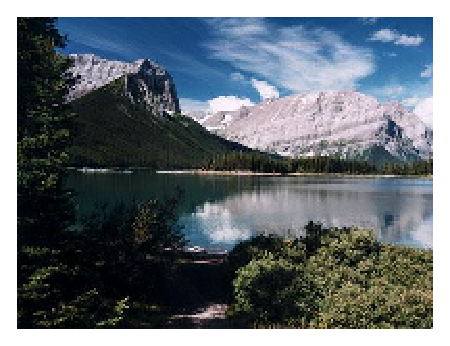
\epsfig{file=kananaskis_small.ps} \raisebox{2.5cm}{\Huge\bf~~~+~} 
\raisebox{0mm}{\epsfig{file=scratchBDD.ps, height=5.3cm, width=3.5cm}}
}}

\vfill

\newpage

\pagenumbering{roman}

\section*{Preface}


The development of {\tt HolBddLib} has gone through two phases.  The
first phase consisted in experiments with different ways of linking
higher order logic (HOL) terms to binary decision diagrams (BDDs).
These are described in the paper {\it Reachability programming in
HOL98 using BDDs\/} \cite{tphols2000-Gordon}. The first release of
\t{HolBddLib}, now called Version~1, consisted of an ad hoc collection
of tools developed for these experiments.  One of the approaches we
experimented with was based on a protected type of `BDD representation
judgements', analogous to the LCF protected type of theorems.
Positive results of Hasan Amjad \cite{Amjad:TPHOLs2001} have lead us
to narrow attention to just this approach. \t{HolBddLib} Version~2,
which is described here, provides a set of representation judgement
rules as core infrastructure for building `fully-expansive' or
`LCF-style' combinations of HOL theorem proving and BDD-based symbolic
calculation algorithms. All higher level tools, such as model
checkers, are programmed in ML as `derived rules'.

The primitive inference rules for representation judgements are in the structure
{\tt{PrimitiveBddRules}}. A few example derived rules are in the
structure {\tt{DerivedBddRules}}. Currently the only derived rules are
ones to compute reachable states and find sequences of transitions to
states with given properties.  It is hoped to soon add a module for
checking properties expressed in the modal $\mu$-calculus (and hence CTL).


Version~1 of {\tt{HolBddLib}} was more elaborate than Version~2
because it mixed together code from a number of experiments.
In Version~1 there was a function, called
{\texttt{termToBdd}}, that tried to represent a \HOL{} term as a BDD
using a dynamically extendable global table mapping \HOL{} terms to
BDDs.  $\t{TermToBdd}$ constructed the BDD of a term $t$ using any
BDDs of subterms of $t$ that were stored in the global table.
{\tt{HolBddLib}} Version~2 has jettisoned this imperative style
in favour of purely functional rules. Some of
the ideas of BDD tables are likely to return in the future, but as
contexts, similar to HOL simpsets, that are passed functionally,
rather than as a single global state held in references.

{\tt{HolBddLib}} Version~1 only supported a single variable
ordering, held in a global variable map. In Version~2, each
representation judgement carries its own variable ordering, so that local
scopes are possible. For convenience, {\tt{DerivedBddRules}}
provides a way of storing a default variable ordering in a global
variable, but this is just a derived facility, not part of the kernel.

{\tt{HolBddLib}} Version~2 adds assumptions to representation judgements
analogous to assumptions of HOL theorems. This enables
Coudert, Berthet and Madre simplification to be represented as a primitive
rule (see the rule \t{BddSimplify} in 
Section~\ref{term-bdd-rules}). 
It also allows the term part
of a representation judgements to be simplified using equations with assumptions
(see the rule \t{BddEqMp} in Section~\ref{BddEqMp}).

{\tt HolBddLib} uses J{\o}rn Lind-Nielsen's \Buddy{} package as a BDD
engine. The interface from \Buddy{} to Moscow ML, called \Muddy, is
due to Ken Friis Larsen and Jakob Lichtenberg, and is described in Part~\ref{muddy}.
{\tt HolBddLib} is built on top of \Muddy{} and
is described in Part~\ref{HolBddLib}.

Some of the material in this document derives from University of
Cambridge Computer Laboratory Technical Report No.~481, December 1999,
by Mike Gordon and Ken Friis Larsen \cite{GordonLarsen}. Although this
report has examples that might be of tutorial use, it has much
obsolete material and methodology deriving for early experiments
pre-dating the release of {\tt HolBddLib} Version~1.


\subsection*{Overview}


In the fully expansive (or `LCF style') approach, theorems are represented by an abstract type
whose primitive operations are the axioms and inference rules of a
logic.  Theorem proving tools are implemented by composing together
the inference rules using ML programs.

This idea can be generalised to computing valid judgements that
represent other kinds of information. In particular, consider
judgements $(a,\rho,t,b)$, where $a$ is a set of boolean terms
(assumptions) that are assumed true, $\rho$ represents a variable
order, $t$ is a boolean term all of whose free variables are boolean
and $b$ is a BDD. Such a judgement is valid if under the assumptions
$a$, the BDD representing $t$ with respect to $\rho$ is $b$, and we
will write \termbdd{a}{\rho}{t}{b} when this is the case.

The derivation of `theorems' like \termbdd{a}{\rho}{t}{b} can be viewed
as `proof' in the style of LCF by defining an abstract type \termbddty{}
that models
judgements $\termbdd{a}{\rho}{t}{b}$ analogously
to the way the type $\ty{thm}$ models theorems $\vdash t$.

\t{HolBddLib} currently contains two main structures: \t{PrimitiveBddRules}
which defines a protected type \termbddty and rules for generating
values of this type, and \t{DerivedBddRules} that contains derived
rules for performing simple fixed-point calculations.  There is also a
theory \t{MachineTransitionTheory} containing the theorems on
reachability and fixed points needed by the derived rules,
and two small subsidiary structures \t{Varmap} and \t{PrintBdd}.


\subsection*{Relation to the Voss system\footnote{Adapted from 
{\it Reachability programming in HOL using BDDs}
\cite{tphols2000-Gordon}}}\label{related}

The Voss system \cite{SegerVoss} has strongly influenced and inspired
the ideas described here. Voss consists of a lazy
ML-like functional language, called FL, with BDDs as a built-in datatype.
Quantified boolean formulae can be input and are parsed to BDDs.
The normal boolean operations $\neg$, $\wedge$, $\vee$, $\equiv$,
$\forall$, $\exists$ are interpreted as BDD operations.  
Algorithms for model checking are easily programmed.

Joyce and Seger interfaced an early HOL system (HOL88) to Voss and in
a pioneering paper showed how to verify complex systems by a
combination of theorem proving deduction and symbolic trajectory
evaluation (STE) \cite{JoyceSeger}. The HOL-Voss system integrates HOL88
deduction with BDD computations.  BDD tools are programmed in FL and
can then be invoked by HOL-Voss tactics, which can make external
calls into the Voss system, passing subgoals via a translation between
the HOL88 and Voss term representations.

In later work Lee, Seger and Greenstreet \cite{LeeGreenstreetSeger}
showed how various optimised BDD algorithms could be programmed in FL.

The early experiments with HOL-Voss suggested that a lighter theorem
proving component was sufficient, since all that was really needed was
a way of combining results obtained from STE. A system based on this
idea, called VossProver, was developed by Carl Seger and his student
Scott Hazelhurst. It provides operations in FL for combining
assertions generated by Voss using proof rules corresponding to the
laws of composition of the temporal logic assertions verified by STE
\cite{hazelhurst-kropfbook-97}.  
VossProver was used to verify
impressive integer and floating-point examples (see the DAC98
paper by Aagaard, Jones and Seger \cite{aagaard-dac-98} for further
discussion and references). 

After Seger and Aagaard moved to Intel, the development of the Voss and
VossProver systems evolved into a new system called Forte.  Only partial details
of this are in the public domain
\cite{oleary-itj-99,aagaard-tphols-99}, but a key idea is that FL is
used both as a specification language and as an LCF-style
metalanguage. The connection between symbolic trajectory evaluation
and proof is obtained via a tactic {\tt{Eval\_tac}} that converts the
result of executing an FL program performing STE into a theorem in the
logic. Theorem proving in Forte is used both to split goals into
smaller subgoals that are tractable for model checking, and to
transform formulae so that they can be checked more efficiently.

The combination of \HOL{} and \Buddy{} in Version~1 of
{\tt{HolBddLib}} provides a somewhat similar programming environment
to Voss's FL (though with eager rather than lazy evaluation and no
special support for STE). \Buddy{} provides BDD operations
corresponding to $\neg$, $\wedge$, $\vee$, $\equiv$, $\forall$,
$\exists$ and the \HOL{} term parser plus \ml{termToBdd} provides a
way of using these to create BDDs from logical terms.  Voss enables
efficient computations on BDDs using functional programming. So does
\ml{HolBddLib}. However, in addition it allows FL-like BDD programming
in ML to be intimately mixed with \HOL{} deduction, so that, for
example, theorem proving tools (e.g.~simplifiers) can be directly
applied to terms to optimise them for BDD purposes (e.g.~disjunctive
partitioning).  This is in line with future developments discussed by
Joyce and Seger \cite{JoyceSeger} and it appears that the Forte system
has similar capabilities.

{\tt{HolBddLib}} Version~2 provides a less developed interactive
programming environment than Version~1. It is more oriented to
providing a clean and simple API allowing implementers to create their
own `fully-expansive' combinations of model checking and theorem
proving. Such a combination could be a Voss-like verification
platform.

\newpage


\makeatletter
\let\My@@tableofcontents\tableofcontents
\renewcommand\tableofcontents{{%
    \let\My@@addvspace\addvspace
    \def\addvspace##1{%
      \@tempskipa##1\relax
      \My@@addvspace{0.1\@tempskipa}%
    }%
    \My@@tableofcontents
}}
\makeatother

\tableofcontents


\pagenumbering{arabic}
\newpage

\part{\Muddy}\label{muddy}

\Muddy is the Moscow
ML interface to \Buddy. It provides ML functions for constructing and
manipulating BDDs via three structures:

\begin{itemize}

\item \t{bdd} defines the ML type
\t{bdd} representing BDDs and associated operations derived from \Buddy;


\item \t{fdd} provides support for blocks of BDD variables
used to encode values representing elements of finite domains;

\item \t{bvec} provides support for Boolean vectors.

\end{itemize}

The current \HolBuddy{} system only uses \t{bdd} and so
the documentation of \t{fdd} and \t{bvec} provided here is minimal
(see Sections~\ref{fdd} and \ref{bvec} below).

\section{Initialisation, termination and tuning sessions}\label{init}

The \Buddy{} package must be initialised before any BDD operations are done.
Initialisation is done with the ML function

\begin{verbatim}
   init : int -> int -> unit
\end{verbatim}\bnind{init}

Evaluating $\t{init}~m~n$ initialises \Buddy{} with $m$ nodes in the
nodetable and a cachesize of $n$.  
The library \t{HolBddLib} (Part~\ref{HolBddLib}) 
initialises the nodetable to 1000000 and cachesize to
be 10000. The following is a quotation from the \Buddy{} documentation \cite{BuDDy}.

\vspace*{-2mm}

{\baselineskip8pt\begin{quote}\footnotesize
Good initial values are

\smallskip

\begin{tabular}{lrr}
{\bf Example} & {\bf nodenum} & {\bf cachesize} \\
Small test examples   & 1000    & 100\\
Small examples        & 10000   & 1000 \\
Medium sized examples & 100000  & 10000\\
Large examples        & 1000000 & 10000
\end{tabular}

\smallskip

Too few nodes will only result in reduced performance and this
increases the number of garbage collections needed. If the package
needs more nodes, then it will automatically increase the size of the
node table.
\end{quote}}

The initial number of nodes is not critical for any BDD operation
as the table will be resized whenever there are too few nodes left
after a garbage collection.  But it does have some impact on the
efficiency of the operations.

The function

\begin{verbatim}
   done : unit -> unit
\end{verbatim}\bnind{done}

frees all memory used by \Buddy{} and resets the
package to its initial state. 

The functions \t{init} and \t{done} should only be called once per session.

The function

\begin{verbatim}
   isRunning : unit -> bool
\end{verbatim}\bnind{isRunning}

tests whether
\Buddy{} is running (i.e.~\t{init} has been called and \t{done} has not been called). It is
useful for checking if initialialisation is needed.

The functions \t{init} and \t{done} should only be called once in a session.

Statistical information from \Buddy{} is available
using the function \t{stats}

\begin{verbatim}
   stats : unit -> {produced     : int,
                    nodenum      : int,
                    maxnodenum   : int,
                    freenodes    : int,
                    minfreenodes : int,
                    varnum       : int,
                    cachesize    : int,
                    gbcnum       : int}
\end{verbatim}\bnind{stats}

The meaning of the values of the various named fields in the record returned by
evaluating \t{stats()} are

\medskip

\begin{tabular}{|l|l|} \hline
{\bf{Field name}}& {\bf{Meaning}}                                              \\ \hline\hline
\t{produced}     & total number of new nodes ever produced                     \\ \hline
\t{nodenum}      & currently allocated number of BDD nodes                     \\ \hline
\t{maxnodenum}   & user defined maximum number of BDD nodes                    \\ \hline
\t{freenodes}    & number of currently free BDD nodes                          \\ \hline
\t{minfreenodes} & minimum number of nodes left after a BDD garbage collection \\ \hline
\t{varnum}       & number of defined BDD variables                             \\ \hline
\t{cachesize}    & number of cache entries                                     \\ \hline
\t{gbcnum}       & number of BDD garbage collections done                      \\ \hline
\end{tabular}

\medskip

The management of the node table and internal caches can be tuned
using the following functions


\begin{verbatim}
   setMaxincrease : int -> int
   setCacheratio  : int -> int
\end{verbatim}\bnind{setMaxincrease}\bnind{setCacheratio}

Evaluating \t{setMaxincrease~$n$} tells \Buddy that the maximum of new nodes added
when doing an expansion of the nodetable should be $n$.  The previous maximum is returned.

Evaluating \t{setCacheratio~$n$} sets the cache ratio to $n$.  
For example, if $n$ is $4$ then the internal caches will a quarter the size of the
nodetable.



\section{BDDs representing {\t{true}} and {\t{false}}}

The atomic BDDs representing the two truthvalues are bound to the ML
identifiers \t{TRUE} and \t{FALSE}, both of type \t{bdd}.

Functions for mapping from ML Booleans to BDDs and vice versa are, respectively

\begin{verbatim}
   fromBool : bool -> bdd
   toBool   : bdd  -> bool
\end{verbatim}\bnind{fromBool}\bnind{toBool}

The function \t{toBool} returns \t{true} on TRUE and \t{false} on FALSE.
It raises the exception \t{Domain} on non-atomic BDDs.

\begin{verbatim}
   equal : bdd -> bdd -> bool
\end{verbatim}\bnind{equal}

tests the equality of two BDDs. Thus \t{TRUE} is \t{equal} to \t{fromBool(true)} and 
\t{FALSE} is \t{equal} to \t{fromBool(false)}.

\section{Variables}

In \Buddy, BDD variables are encoded as integers (type \t{int} in ML) and the BDD variable ordering
is the numerical ordering. Thus to build a BDD to represent a \HOL{} term with a
particular variable ordering it is necessary to map \HOL{} variables to
integers so that the numerical order corresponds to the desired
variable order.

The number of variables in use must be declared using

\begin{verbatim}
   setVarnum : int -> unit
\end{verbatim}\bnind{setVarnum}

Evaluating $\t{setVarnum}~n$ declares that the $n$ variables $0$,
$1$, $\ldots$ , $n{-}1$ are available for use. The number of variables
can be increased dynamically during a session by calling \t{setVarnum}
with a larger number. The number of variables cannot be decreased
dynamically. The function

\begin{verbatim}
   getVarnum : unit -> int
\end{verbatim}\bnind{getVarnum}

returns the number of variables in use (i.e.~the argument of the last
application of \t{setVarnum}).

The function

\begin{verbatim}
   ithvar : int -> bdd
\end{verbatim}\bnind{ithvar}

maps an ML integer to a BDD that consists of just the variable
corresponding to the integer and

\begin{verbatim}
   nithvar : int -> bdd
\end{verbatim}\bnind{nithvar}

maps
an integer to the BDD representing the negation of the variable.

Note that evaluating $\t{ithvar}~n$ or $\t{nithvar}~n$ will raise the exception
\t{Fail} (with string argument \texttt{"Unknown variable"})
if $n$ has not been declared as in use, i.e.~if
$\t{setVarnum}~m$ has not been previously evaluated for some $m$
greater than $n$.


\section{Sets of variables and quantification}\label{varSet}

\Buddy{} provides operations on BDDs for quantifying with respect to sets
of variables. The module  \t{bdd} provides a type \t{varSet} to represent such
sets with, respectively, a constructor and two destructors:

\begin{verbatim}
   makeset : int list -> varSet
   scanset : varSet   -> int vector
   fromSet : varSet   -> bdd
\end{verbatim}\bnind{makeset}\bnind{scanset}\bnind{fromSet}

The destructor \t{scanset} returns a vector of the variables in the
set and the destructor \t{fromSet} returns a BDD representing the
conjunction of the variables in the set.

The following functions quantify BDDs with respect to sets of variables:

\begin{verbatim}
   forall : varSet -> bdd -> bdd
   exist  : varSet -> bdd -> bdd
\end{verbatim}\bnind{forall}\bnind{exist}

\section{Assignments, composition, replacement and restriction}\label{replace}

\Muddy provides a function for general purpose simultaneous
substitution of arbitrary BDDs for variables in a given BDD (\t{veccompose}). It also
provides and three optimised special cases: substituting for a single
variable (\t{compose}), renaming variables (\t{replace}) and
substituting with boolean constants (\t{restrict}).

The operation \t{veccompose} performs the simultaneous substitution 
of BDDs for variables in a BDD. The argument of \t{veccompose}
is a value of type \t{composeSet}\tyind{composeSet} 
(created with a constructor \t{composeSet})
that specifies a list if pairs \t[(($n_1$,$b_1$),$\ldots$,, where BDD variable $n$ is to be pre

\begin{verbatim}
   composeSet : (int * bdd) list -> composeSet
   veccompose : composeSet -> bdd -> bdd
\end{verbatim}\bnind{composeSet}\bnind{veccompose}

A single variable can be replaced with a BDD using

\begin{verbatim}
   compose : bdd -> bdd -> int -> bdd
\end{verbatim}\bnind{compose}

Evaluating \t{compose~$b_1$~$b_2$~$n$} substitutes $b_2$ for the
variable $n$ in $b_1$.

Variables can be renamed using the function \t{replace} that takes
an argument of type \t{pairSet}\tyind{pairSet} representing sets of pairs of variables
(with constructor \t{makepairSet})

\begin{verbatim}
   makepairSet : (int * int)list -> pairSet
   replace     : bdd -> pairSet -> bdd
\end{verbatim}\bnind{makepairSet}\bnind{replace}

Evaluating \t{makepairSet[($x_1$,$x_1'$), $\ldots$ , ($x_n$,$x_n'$)]}
creates a set of pairs specifying that $x_i'$ be substituted for $x_i$
(for $1\leq i\leq n$).  A renaming with \t{replace} will fail if it
would result in distinct variables being identified (i.e.~if the shape of the BDD would change).

BDDs can be restricted by instantiating variables to {\t{TRUE}} or
{\t{FALSE}} using the function \t{restrict} that takes
as argument a value of type \t{assignment}\tyind{assignment} 
(which has a constructor \t{assignment} and destructor \t{getAssignment}).

\begin{verbatim}
   assignment    : (int * bool)list -> assignment
   getAssignment : assignment -> (int * bool) list
   restrict      : bdd -> assignment -> bdd
\end{verbatim}\bnind{restrict}\bnind{assignment}\bnind{getAssignment}

Evaluating \t{assignment[($v_1$,$t_1$), $\ldots$ , ($v_n$,$t_n$)]}
creates an assignment specifying that each $v_i$ be instantiated to
$\t{fromBool(}t_i\t{)}$ (for $1{\leq}i{\leq}n$). 


\section{Finding satisfying assignments}

An assignment satisfying a BDD can be computed via \Buddy using

\begin{verbatim}
   satone : bdd -> assignment
\end{verbatim}\bnind{makeset}\bnind{scanset}\bnind{fromSet}

The exception \t{Domain} is raised if the argument to \t{satone} is unsatisfiable.

\newpage
Alternatively, a model can be computed by an ML program such as:

\begin{verbatim}
   val findSat =
    let fun findSatAux bdd = 
         if bdd.equal bdd bdd.TRUE
          then []
          else
           if bdd.equal bdd bdd.FALSE
            then raise Domain
            else
             ((bdd.var bdd,true) :: findSatAux(bdd.high bdd) 
              handle Domain =>
              (bdd.var bdd, false) :: findSatAux(bdd.low bdd))
    in
     assignment o findSatAux
    end;
\end{verbatim}

The functions \t{satone} and \t{findSat} do not necessarily find the
same satisfying assignment, if more than one exists. Also,
\t{findSat} stops when it has found enough variable bindings to
satisfy the BDD, so may not return an assignment giving values to all
the variables.

\section{Boolean operations on BDDs}\label{app}

The structure \t{bdd} introduces a type \t{bddop}
corresponding to Boolean operations on BDDs. 
The ML function

\begin{verbatim}
   apply : bdd -> bdd -> bddop -> bdd
\end{verbatim}\bnind{apply}

applies a BDD operation to BDD values.

\Buddy{} provides functions for calculating in a single step the
result of performing a Boolean operation and then quantifying the
result with respect to several variables.

\begin{verbatim}
   appall : bdd -> bdd -> bddop -> varSet -> bdd
   appex  : bdd -> bdd -> bddop -> varSet -> bdd
\end{verbatim}\bnind{appall}\bnind{appex}

The function \t{appall} universally quantifies the result of the
Boolean operation and \t{appex} existentially quantifies it.

\Muddy{} provides ten operations of type \t{bddop} and for each of
these an ML infix, pre-defined using \t{apply}, of type \t{bdd~*~bdd~->~bdd}.



\begin{center}

\begin{tabular}{|l||l|l|} \hline
\t{bddop}\bnind{bddop} & \t{bdd~*~bdd~->~bdd} & Result of applying to $(b_1,b_2)$\\ \hline\hline
\t{And}\bnind{And} & \t{AND} & $b_1\wedge b_2$ \\ \hline
\t{Nand}\bnind{Nand} & \t{NAND} & $\neg(b_1\wedge b_2)$ \\ \hline
\t{Or}\bnind{Or}  & \t{OR} & $b_1\vee b_2$ \\ \hline
\t{Nor}\bnind{Nor} & \t{NOR} & $\neg(b_1\vee b_2)$ \\ \hline
\t{Biimp}\bnind{Biimp} & \t{BIIMP} & $b_1= b_2$ \\ \hline
\t{Xor}\bnind{Xor} & \t{XOR} & $\neg(b_1=b_2)$ \\ \hline
\t{Imp}\bnind{Imp} & \t{IMP} & $b_1\imp b_2$ \\ \hline
\t{Invimp}\bnind{Invimp} & \t{INVIMP} & $b_2\imp b_1$ \\ \hline
\t{Lessth}\bnind{Lessth} & \t{LESSTH} & $\neg b_1\wedge b_2$ \\ \hline
\t{Diff}\bnind{Diff} & \t{DIFF} & $b_1\wedge \neg b_2$ \\ \hline
\end{tabular}\label{bddops}

\end{center}

\Muddy{} also provides a unary negation operator and ternary conditional operator.

\begin{verbatim}
   NOT : bdd -> bdd
   ITE :  bdd -> bdd -> bdd -> bdd
\end{verbatim}\bnind{NOT}\bnind{ITE}

$\t{NOT}~b$ is the BDD corresponding to  `$\neg b$' and $\t{ITE}~b~b_1~b_2$ is the BDD corresponding
to `$if~b~then~b_1~else~b_2$'.




\section{Inspecting and counting nodes and states}

The integer labelling a BDD node and the BDDs corresponding to the high
(i.e.~{\t{true}}) and low (i.e.~{\t{false}}) nodes are obtained,
respectively, with

\begin{verbatim}
   var  : bdd -> int
   high : bdd -> bdd
   low  : bdd -> bdd
\end{verbatim}\bnind{var}\bnind{high}\bnind{low}

Thus if $b$ is the BDD of ``${\it{if}}~x~{\it{then}}~t_1~{\it{else}}~t_2$''
then $\t{var}~b$ will return the number representing variable $x$,
$\t{high}~b$ will return the BDD of $t_1$ and $\t{low}~b$ will return
the BDD of $t_2$.

Note that \t{var}, \t{high} and \t{low} raise an exception if applied
to \t{TRUE} or \t{FALSE}.

The entire \Buddy{} node table of a BDD can be copied into ML using

\begin{verbatim}
   nodetable : bdd -> int * (int * int * int)vector
\end{verbatim}\bnind{nodetable}

The integer returned as the first component of the pair is a pointer
(starting from 0) into the second component, a vector of node
descriptors. This pointer points to the root node. Each node
descriptor is a triple of integers $(v,l,h)$, where $v$ is the node
label (i.e.~a number representing a variable), $l$ points to the low
({\t{false}}) node in the vector and $h$ points to the high
({\t{true}}) node. The first two nodes in the vector are special:
they represent {\t{true}} and {\t{false}}, respectively, and arbitrarily have
the structure $(0,0,0)$.

The number of nodes in a BDD is computed by the function

\begin{verbatim}
   nodecount : bdd -> int
\end{verbatim}\bnind{nodecount}

This could be defined by

\begin{verbatim}
   fun nodecount bdd = Vector.length(snd(nodetable bdd));
\end{verbatim}

However, \t{nodecount} defined this way is likely to run out of space
on large BDDs (since it involves copying the argument BDD from
\Buddy's representation into an ML vector).  Thus the ML function
provided by \Muddy{} invokes \Buddy's \t{nodecount} function directly
and so is space-efficient.

The number of assignments {\it to all variables in use in the current
session\/} that satisfy a BDD (i.e.~make it true) is given by the ML
function

\begin{verbatim}
   satcount : bdd -> real
\end{verbatim}\bnind{satcount}

The answer is exact until the result is too big to be represented as a
Moscow ML integer. Real numbers are used so that results can be
returned when this happens.

The function

\begin{verbatim}
   support : bdd -> varSet
\end{verbatim}\bnind{support}

gives the variables that a BDD depends on. 

An application is to define
a function that counts the number of valuations of a BDD using
\t{satcount}.

\begin{verbatim}
   statecount : bdd -> real
\end{verbatim}\bnind{statecount}

The
definition of \t{statecount} is

\begin{verbatim}
fun statecount bdd =
 let val sat    = satcount bdd
     val total  = Real.fromInt(getVarnum())
     val sup    = scanset(support bdd)
     val numsup = Real.fromInt(Vector.length sup)
     val free   = total - numsup
 in 
  if equal bdd TRUE 
   then 0.0
   else sat / Math.pow(2.0, free)
 end
\end{verbatim}

If a BDD is representing a set of states, then \t{statecount} gives
the number of states in the set (hence the name).


\section{Coudert, Berthet \& Madre simplification}

The ML function

\begin{verbatim}
   simplify : bdd -> bdd -> bdd
\end{verbatim}\bnind{simplify}

simplifies its second argument under the assumption that the first
argument is true. Thus evaluating
\t{simplify~$b_1$~$b_2$} results in a BDD $b_2'$, hopefully simpler than $b_2$, such that
$b_1 \Imp (b_2 = b_2')$ or, equivalently, \mbox{$b_1 \wedge b_2 = b_1 \wedge b_2'$}.
More precisely,
the relationship between $b_1$, $b_2$ and $b_2'$ is that
the BDD \t{IMP($b_1$,BIIMP($b_2$,$b_2'$))} is the BDD \t{TRUE}
(or, equivalently, that \t{AND($b_1$,$b_2$)} and \t{AND($b_1$,$b_2'$)}
are \t{equal}, i.e.~the same BDD).

For more details see Henrik Reif Andersen's lecture
notes on BDDs \cite{HenrikNotes}, where
the algorithm underlying \t{simplify} is described and attributed to a paper by
Coudert, Berthet and Madre \cite{CoudertBerthetMadre}.

\section{Saving, hashing and printing BDDs}\label{printing}

BDDs can be saved on disk with the functions

\begin{verbatim}
   bddSave : string -> bdd -> unit
   bddLoad : string -> bdd
\end{verbatim}\bnind{bddSave}\bnind{bddLoad}

The string argument is a file name.

\Buddy{} provides two ways of printing BDDs: (i) as the set of paths from
the root node to the {\it{true}} node and (ii) to the format used by
the \t{dot} graph drawing
program\footnote{\tt{http://www.research.att.com/sw/tools/graphviz/}}.

The function

\begin{verbatim}
   hash : bdd -> int
\end{verbatim}\bnind{hash}

hashes a bdd to an integer.

The functions for printing BDDs are;

\begin{verbatim}
   printset   : bdd -> unit
   printdot   : bdd -> unit
   fnprintset : string -> bdd -> unit
   fnprintdot : string -> bdd -> unit
\end{verbatim}\bnind{printset}\bnind{printdot}\bnind{fnprintset}\bnind{fnprintdot}

\t{printset} and \t{printdot} print to standard output, whilst
\t{fnprintset} and \t{fnprintdot} print to a file with the supplied
name.

\t{printset} and \t{fnprintset} print out a sequence of paths, each one having the form

\smallskip

~$\t{}<m_0\t{:}n_0\t{,} \ldots \t{,} m_l\t{:}n_l\t{>}$

\smallskip

where the $n_0$, $\ldots$ , $n_l$ after the colon (\t{:}) are \t{0} or
\t{1} and indicate that the next node in the path is reached by
following the low ({\t{false}}) or high ({\t{true}}) pointer,
respectively. 

For
example, evaluating

\smallskip
~\t{printset~(AND(ithvar~0,~OR(ithvar~1,~NOT(ithvar~2))))}
\smallskip

results in

\smallskip
~\t{<0:1,~1:0,~2:0><0:1,~1:1>}
\smallskip

which is best understood by looking at the diagram of the BDD drawn by
\t{dot} that appears below.

To illustrate printing to \t{dot} format,  the same BDD can be
printed to a file \t{ex} by evaluating

\smallskip
~\t{fnprintdot~"ex"~(AND(ithvar~0,~OR(ithvar~1,~NOT(ithvar~2))))}
\smallskip

executing ~\t{dot~-Tps~ex~>~ex.ps} (in Unix) results in
the following Postscript diagram of a BDD

\begin{center}
\epsfig{file=ex.ps, height=5cm, width=3cm} 
\end{center}

\section{Dynamic variable reordering}

\Buddy{} provides functions for dynamic variable reordering using a variety of methods.
See the \Buddy{} documentation \cite{BuDDy} for further details. The dynamic reordering
types and functions provided in ML via \Muddy{} are in the structure \t{bdd} and are

{\footnotesize\begin{verbatim}
    eqtype fixed
    FIXED            : fixed
    FREE             : fixed

    addvarblock      : varnum -> varnum -> fixed -> unit
    clrvarblocks     : unit -> unit

    eqtype method
    WIN2             : method
    WIN2ITE          : method
    SIFT             : method
    SIFTITE          : method
    RANDOM           : method
    REORDER_NONE     : method

    reorder          : method -> unit
    autoReorder      : method -> method
    autoReorderTimes : method -> int -> method

    getMethod        : unit -> method
    getTimes         : unit -> int

    disableReorder   : unit -> unit
    enableReorder    : unit -> unit

    varToLevel       : varnum -> int
    varAtLevel       : int -> varnum
\end{verbatim}}

\section{The \Muddy{} structure \t{fdd}}\label{fdd}

The structure \t{fdd} provides functions for manipulating values of finite domains.
Functions are provided to allocate blocks of BDD variables to represent integer values instead
of only Booleans.

Encoding is done with the least significant bits first in the BDD ordering. For example, if variables
$v_0, v_1, v_2, v_3$ are used to encode $12$, then the encoding would yield
$v_0=0$, $v_1=0$, $v_2=1$ and $v_3=1$.

See the \Buddy{} documentation \cite{BuDDy} for further details. See the ML structure \t{fdd}
for the \Buddy{} facilities provides in ML via \Muddy:

{\footnotesize\begin{verbatim}
   type fddvar

   extDomain  : int list -> fddvar list
   clearAll   : unit -> unit
   domainNum  : unit -> int
   domainSize : fddvar -> int
   varNum     : fddvar -> int
   vars       : fddvar -> bdd.varnum list
   ithSet     : fddvar -> bdd.varSet
   domain     : fddvar -> bdd.bdd
   setPairs   : (fddvar * fddvar) list -> bdd.pairSet
\end{verbatim}}

\section{The \Muddy{} structure \t{bvec}}\label{bvec}

The structure \t{bvec} provides tools for encoding integers as arrays
of BDDs, where each BDD represents one bit of an expression.

See the \Buddy{} documentation \cite{BuDDy} for further details. See the ML structure \t{bvec}
for the \Buddy{} facilities provides in ML via \Muddy{}.

{\footnotesize
\begin{verbatim}
   type bvec

   bvectrue    : fdd.precision -> bvec 
   bvecfalse   : fdd.precision -> bvec 
   con         : fdd.precision -> int -> bvec
   var         : fdd.precision -> bdd.varnum -> int -> bvec
   varfdd      : fdd.fddvar -> bvec

   coerce      : fdd.precision -> bvec -> bvec

   isConst     : bvec -> bool
   getConst    : bvec -> int
   lookupConst : bvec -> int option

   add         : bvec * bvec -> bvec
   sub         : bvec * bvec -> bvec
   mul         : bvec * bvec -> bvec
   mulfixed    : bvec * int -> bvec
   div         : bvec * bvec -> bvec * bvec
   divfixed    : bvec * int -> bvec * bvec
   divi        : bvec * bvec -> bvec
   divifixed   : bvec * int -> bvec

   modu        : bvec * bvec -> bvec
   modufixed   : bvec * int -> bvec
   shl         : bvec -> bvec -> bdd.bdd -> bvec
   shlfixed    : bvec -> int -> bdd.bdd -> bvec
   shr         : bvec -> bvec -> bdd.bdd -> bvec
   shrfixed    : bvec -> int -> bdd.bdd -> bvec

   lth         : bvec * bvec -> bdd.bdd
   lte         : bvec * bvec -> bdd.bdd
   gth         : bvec * bvec -> bdd.bdd
   gte         : bvec * bvec -> bdd.bdd
   equ         : bvec * bvec -> bdd.bdd
   neq         : bvec * bvec -> bdd.bdd
\end{verbatim}}

\section{Storage allocation and garbage collection}
\label{sec:technical-details}

The heart of the \Muddy package is mostly stub code that mirrors the
\Buddy API and takes care of translating C values into SML values and
vice versa.

The most tricky part is to make the \mosml garbage collector cooperate
with the \Buddy garbage collector (we don't want either collector to
try to collect the other's garbage).  The cooperation is done by using
the \emph{finalized values} facility of the \mosml runtime system.
That is, whenever a \texttt{bdd} value is returned from the \Buddy
library, \Muddy register it as an external root (via
\verb+bdd_addref+) and wraps it into a finalized value.  

A finalized value, in the \mosml runtime system, is a pair where the
first component is the \emph{destructor} (a function pointer) and the
second component is the \emph{data} (typicaly a pointer).  When the
\mosml collector collect a finalized value it apply the destructor on
the data.  In the case of the \Muddy package the destructor is
\verb+bdd_delref+ and the data is the node-index returned by \Buddy.

Output showing the activation of the \Buddy garbage collector can be generated
using the function

\begin{verbatim}
   verbosegc : (string * string) option -> unit
\end{verbatim}\bnind{verbosegc}

Evaluating \t{verbosegc(SOME($pregc$,$postgc$))} instructs BuDDy to print
$pregc$ when a BuDDy GC is initiated and print $postgc$ when the
\Buddy GC is completed.

\newpage

\part{Description of \t{HolBddLib}}\label{HolBddLib}

\t{HolBddLib} currently consists of five modules

\begin{enumerate}
\item \t{Varmap} defines the ML type \t{varmap} that represents mappings,
often denoted by $\rho$,
from HOL variables to BDD variables;

\item \t{PrintBdd} provides rudimentary facilities for printing
BDDs with respect to a varmap;

\item \t{PrimitiveBddRules} defines the protected type \termbddty
representing BDD representation judgements \termbdd{a}{\rho}{t}{b}
with the semantics that under assumptions $a$, term $t$ is represented by BDD $b$ with respect to
varmap $\rho$;

\item \t{DerivedBddRules} defines some derived rules for computing
the representation of the reachable states of a transition system,
and also for finding shortest paths to states  satisfying a given property;

\item \t{MachineTransitionTheory} contains HOL reachability and fixedpoint theorems needed
for the derived rules in  \t{DerivedBddRules}.


\end{enumerate}


Executing

\vspace*{-2mm}

\begin{verbatim}
   load "HolBddLib";
\end{verbatim}

\vspace*{-2mm}

loades these five modules and
initialises \Buddy{} with a nodesize of 1000000
and cachesize of 10000.  

If you want to perform your own \Buddy{} initialisation with different
values, then instead of loading \t{HolBddLib}, load \t{bdd} and then
call \t{bdd.init} with the parameters you want (see
Section~\ref{init}).  \t{PrimitiveBddRulesTheory} and/or
\t{MachineTransitionTheory} etc.~can  then be loaded.

\section{The structure \ml{Varmap}}\label{Varmap}

The type \t{varmap} is defined by

\vspace*{-2mm}

\begin{verbatim}
   type varmap = (string, int) Binarymap.dict
\end{verbatim}\tyind{varmap}

\vspace*{-2mm}

Strings are the names of HOL boolean variables and the integers associated with them
are the corresponding BDD variables.

The following operations and predicates on varmaps are provided:

\begin{verbatim}
   empty   : varmap
   insert  : string * int -> varmap -> varmap
   remove  : string -> varmap -> varmap
   peek    : varmap -> string -> int option
   dest    : varmap -> (string * int) list
   eq      : varmap * varmap -> bool
   size    : varmap -> int
   extends : varmap -> varmap -> bool
   unify   : varmap -> varmap -> varmap
\end{verbatim}%
\bnind{Varmap.empty}%
\bnind{Varmap.insert}%
\bnind{Varmap.remove}%
\bnind{Varmap.peek}%
\bnind{Varmap.dest}%
\bnind{Varmap.eq}%
\bnind{Varmap.size}%
\bnind{Varmap.extends}%
\bnind{Varmap.unify}%


with the semantics

\bigskip

\begin{tabular}{|l|l|} \hline
\t{Varmap.empty} &    the empty varmap \\ \hline
\t{Varmap.insert} &   add an entry \\ \hline
\t{Varmap.remove} &   delete an entry for a variable \\ \hline
\t{Varmap.peek} &     lookup the value of a variable \\ \hline
\t{Varmap.dest} &     convert to a list of pairs \\ \hline
\t{Varmap.eq} &       pointer equality of varmaps ({\it not} general equality) \\ \hline
\t{Varmap.size} &     number of entries \\ \hline
\t{Varmap.extends} &  test if first argument included in second argument\\ \hline
\t{Varmap.unify} &  compute smallest varmap that extends both arguments\\ \hline
\end{tabular}

\section{The structure \ml{PrintBdd}}\label{PrintBdd}

\t{PrintBdd} builds on top of \Muddy's support for drawing BDDs using the \t{dot}
program (see Section~\ref{printing}). Three functions are provided.

\begin{verbatim}
   dotBdd             : string -> string -> bdd -> bdd
   dotLabelledTermBdd : string -> string -> term_bdd -> unit
   dotTermBdd         : term_bdd -> unit
\end{verbatim}%
\bnind{dotBdd}%
\bnind{dotLabelledTermBdd}%
\bnind{dotTermBdd}%

\begin{description}
\item[$\t{dotBdd}~file~label~bdd$]\mbox{}\\
prints the BDD $bdd$ to $file$\t{.dot} with
the label being the string $label$. The BDD variables are printed as the numbers used by \Buddy.
The \t{dot} program is then invoked to create 
a postscript file $file$\t{.ps}. The argument BDD is returned.

\item[$\t{dotLabelledTermBdd}~file~label~tb$]\mbox{}\\
prints the
BDD part of \termbddty $tb$ with the nodes labelled with
the variables specified in the varmap part of $tb$. A file $file$\t{.ps}
is created, and the BDD is labelled with the string $label$.


\item[$\t{dotTermBdd}~tb$]\mbox{}\\
prints the
BDD part of \termbddty $tb$ with the nodes labelled with
the variables specified in the varmap part of $tb$. A file \t{ScratchBdd.ps}
is created, and the BDD is labelled by default with a representation
of the term part of $tb$. The default labels
can be suppressed (i.e. set to be always the empty string) by assigning \t{false}
to the global reference \t{dotTermBddFlag}.
\end{description}

\section{The structure \t{PrimitiveBddRules}}\label{PrimitiveBddRules}

The structure \ml{PrimitiveBddRules} defines the type \termbddty{} by

\vspace*{-2mm}

\begin{verbatim}
   type assums = term HOLset.set;
   datatype term_bdd = TermBdd of assums * varmap * term * bdd;
\end{verbatim}\tyind{term\_bdd}\tyind{assums}

\vspace*{-2mm}

The constructor \t{TermBdd} is not exported, so the only way to construct
values of type \termbddty is using the following inference rules
(which are described in more detail in the rest of this section).

{\footnotesize\begin{verbatim}
   BddExtendVarmap           : term_bdd->varmap->term_bdd
   BddFreevarsContractVarmap : term->term_bdd->term_bdd
   BddSupportContractVarmap  : term->term_bdd->term_bdd
   BddVar                    : bool->varmap->term->term_bdd
   BddCon                    : bool->varmap->term_bdd
   BddNot                    : term_bdd->term_bdd
   BddIte                    : term_bdd*term_bdd*term_bdd->term_bdd
   BddOp                     : bddop*term_bdd*term_bdd->term_bdd
   BddForall                 : term list->term_bdd->term_bdd
   BddExists                 : term list->term_bdd->term_bdd
   BddAppall                 : term list->bddop*term_bdd*term_bdd->term_bdd
   BddAppex                  : term list->bddop*term_bdd*term_bdd->term_bdd
   BddCompose                : term_bdd*term_bdd->term_bdd->term_bdd
   BddListCompose            : (term_bdd*term_bdd)list->term_bdd->term_bdd
   BddRestrict               : (term_bdd*term_bdd)list->term_bdd->term_bdd
   BddReplace                : (term_bdd*term_bdd)list->term_bdd->term_bdd
   BddEqMp                   : thm->term_bdd->term_bdd
   BddSimplify               : term_bdd*term_bdd->term_bdd
\end{verbatim}}

Destructor functions \t{dest\_term\_bdd}, \t{getAssums}, \t{getVarmap}, \t{getTerm}
and \t{getBdd} for values of type \termbddty are described in Section~\ref{misc}

There is also a single oracle function
\t{BddThmOracle} that derives the HOL theorem $a \vdash t$
from the representation judgement \termbdd{a}{\rho}{t}{\ml{TRUE}}
(details are in Section~\ref{oracle}).

Many of the rules assume that the varmaps in their \termbddty
arguments are all equal. To apply these rules to hypotheses with
different varmaps it may be possible to use \t{BddExtendVarmap},
\t{BddFreevarsContractVarmap} or \t{BddSupportContractVarmap} to make
the varmaps equal.  It is expected that derived rules to enable
judgements with different varmaps to be combined will be implemented,
however, as the soundness conditions for these are potentially subtle,
such rules have not been included in the `trusted kernel'.

Currently we have no formal treatment of notions of soundness or
completeness for the rules in \t{PrimitiveBddRules}, though this is
being thought about. We think the rules are `obviously sound', but
such intuitions are known to be unreliable! Our intuition about
completeness is weaker: it is probable that as more experience with
derived rules is obtained, the need for additional primitive rules
will appear. Support for `local scopes' (combining judgements with
different variable orders) is an area that may reveal incompleteness
in the current rules.

\subsection{Rules for generating representation judgements}\label{term-bdd-rules}

The notation $a_1 \cup a_2$ denotes the union of $a_1$ and $a_2$ 
Assumptions of
representation judgements are identified up to $\alpha$-conversion (as
are assumptions of HOL theorems).
The implementation is $a_1 \cup a_2~=~\t{HOLset.union}~a_1~a_2$. 
The empty set of assumptions is denoted by \emptyass, a set of
assumptions containing terms $t_1, \ldots ,t_n$ is denoted by
$\setass{t_1, \ldots ,t_n}$  and 
$\termbdd{\emptyass}{\rho}{t}{b}$ is abbreviated to
$\termbdd{}{\rho}{t}{b}$.


\subsubsection*{Extending and contracting the varmap}

\newsavebox\BddExtendVarmap
\begin{lrbox}\BddExtendVarmap
\begin{minipage}{\minipagewidth}

\begin{footnotesize}
{\verb+BddExtendVarmap : varmap -> term_bdd -> term_bdd +}
\end{footnotesize}
\vspace*{-3mm}

\noindent \rule\minipagewidth{0.1pt}

\vspace*{-2mm}

$$\begin{array}{c}
{\footnotesize\t{Varmap.extends}}~\rho_1~\rho_2 \qquad \termbdd{a}{\rho_1}{t}{b} 
\\ \hline
\termbdd{a}{\rho_2}{t}{b}
\end{array}$$

\noindent \rule\minipagewidth{0.1pt}

\begin{footnotesize}
Raises \t{BddExtendVarmapError} if $\rho_2$ doesn not extend $\rho_1$
\end{footnotesize}
\end{minipage}
\end{lrbox}
\fbox{\usebox{\BddExtendVarmap}}\bnind{BddExtendVarmap}

\bigskip

\newsavebox\BddFreevarsContractVarmap
\begin{lrbox}\BddFreevarsContractVarmap
\begin{minipage}{\minipagewidth}

\begin{footnotesize}
{\verb+BddFreevarsContractVarmap : term -> term_bdd -> term_bdd +}
\end{footnotesize}
\vspace*{-3mm}

\noindent \rule\minipagewidth{0.1pt}

\vspace*{-2mm}

$$\begin{array}{c}
\termbdd{a}{\rho}{t}{b} \qquad \mbox{$v$ not free in $t$}
\\ \hline
\termbdd{a}{({\footnotesize{\texttt{Varmap.remove~"}}}v{\footnotesize{\texttt{"}}}~\rho)}{t}{b}
\end{array}$$

\noindent \rule\minipagewidth{0.1pt}

\begin{footnotesize}
Raises \t{BddFreevarsContractVarmapError} if $v$ not free in $t$
\end{footnotesize}
\end{minipage}
\end{lrbox}
\fbox{\usebox{\BddFreevarsContractVarmap}}\bnind{BddFreevarsContractVarmap}



\bigskip

\newsavebox\BddSupportContractVarmap
\begin{lrbox}\BddSupportContractVarmap
\begin{minipage}{\minipagewidth}

\begin{footnotesize}
{\verb+BddSupportContractVarmap : term -> term_bdd -> term_bdd +}
\end{footnotesize}
\vspace*{-3mm}

\noindent \rule\minipagewidth{0.1pt}

\vspace*{-2mm}

$$\begin{array}{c}
\termbdd{a}{\rho}{t}{b} \qquad \mbox{$\rho(v)$ does occur in $b$}
\\ \hline
\termbdd{a}{({\footnotesize{\texttt{Varmap.remove~"}}}v{\footnotesize{\texttt{"}}}~\rho)}{t}{b}
\end{array}$$

\noindent \rule\minipagewidth{0.1pt}

\begin{footnotesize}
Raises \t{BddSupportContractVarmapError} if $\rho(v)$ not in the support of $b$
\end{footnotesize}
\end{minipage}
\end{lrbox}
\fbox{\usebox{\BddSupportContractVarmap}}\bnind{BddSupportContractVarmap}


\subsubsection*{Variables and constants}

\newsavebox\BddVar
\begin{lrbox}\BddVar
\begin{minipage}{\minipagewidth}

\begin{footnotesize}
{\verb+BddVar : bool -> varmap -> term -> term_bdd  +}
\end{footnotesize}
\vspace*{-3mm}

\noindent \rule\minipagewidth{0.1pt}

\vspace*{-2mm}

$$\begin{array}{c}
\begin{array}{c}
\rho(v)=n
\\ \hline
\termbdd{}{\rho}{v}{{\footnotesize\t{ithvar}}~n}
\end{array} ~\footnotesize{\t{BddVar~true}}

\\[8mm]

\begin{array}{c}
\rho(v)=n
\\ \hline
\termbdd{}{\rho}{v}{{\footnotesize\t{nithvar}}~n}
\end{array}~ {\footnotesize\t{BddVar~false}}

\end{array}$$

\noindent \rule\minipagewidth{0.1pt}

\begin{footnotesize}
Raises \t{BddVarError} if $v$ not in the domain of $\rho$
\end{footnotesize}
\end{minipage}
\end{lrbox}
\fbox{\usebox{\BddVar}}\bnind{BddVar}

\bigskip

\newsavebox\BddCon
\begin{lrbox}\BddCon
\begin{minipage}{\minipagewidth}

\begin{footnotesize}
{\verb+BddCon : bool -> varmap -> term_bdd  +}
\end{footnotesize}
\vspace*{-3mm}

\noindent \rule\minipagewidth{0.1pt}

\vspace*{-2mm}

$$\begin{array}{c}
\begin{array}{c}

\\ \hline
\termbdd{}{\rho}{{\footnotesize\t{T}}}{{\footnotesize\t{TRUE}}}
\end{array} ~\footnotesize{\t{BddCon~true}}

\\[8mm]

\begin{array}{c}
\\ \hline
\termbdd{}{\rho}{{\footnotesize\t{F}}}{{\footnotesize\t{FALSE}}~n}
\end{array}~ {\footnotesize\t{BddCon~false}}

\end{array}$$

\noindent \rule\minipagewidth{0.1pt}

\begin{footnotesize}
Always succeeds
\end{footnotesize}
\end{minipage}
\end{lrbox}
\fbox{\usebox{\BddCon}}\bnind{BddCon}

\subsubsection*{Boolean operations}



\newsavebox\BddNot
\begin{lrbox}\BddNot
\begin{minipage}{\minipagewidth}

\begin{footnotesize}
{\verb+BddNot : term_bdd -> term_bdd +}
\end{footnotesize}
\vspace*{-3mm}

\noindent \rule\minipagewidth{0.1pt}

\vspace*{-2mm}

$$\begin{array}{c}
\termbdd{a}{\rho}{t}{b}
\\ \hline
\termbdd{a}{\rho}{\neg t}{{\footnotesize\t{NOT}}~b}
\end{array}$$

\noindent \rule\minipagewidth{0.1pt}

\begin{footnotesize}
Always succeeds
\end{footnotesize}
\end{minipage}
\end{lrbox}
\fbox{\usebox{\BddNot}}\bnind{BddNot}

\bigskip

\newsavebox\BddIte
\begin{lrbox}\BddIte
\begin{minipage}{\minipagewidth}

\begin{footnotesize}
{\verb+BddIte : term_bdd * term_bdd * term_bdd -> term_bdd +}
\end{footnotesize}
\vspace*{-3mm}

\noindent \rule\minipagewidth{0.1pt}

\vspace*{-2mm}

$$\begin{array}{c}
\termbdd{a}{\rho}{t}{b} \qquad \termbdd{a_1}{\rho}{t_1}{b_1} \qquad \termbdd{a_2}{\rho}{t_2}{b_2}
\\ \hline
\termbdd{a \cup a_1 \cup a_2}{\rho}{\mbox{\footnotesize\t{(if~$t$~then~$t_1$~else~$t_2$)}}}{{\footnotesize\t{ITE}}~b~b_1~b_2}
\end{array}$$

\noindent \rule\minipagewidth{0.1pt}

\begin{footnotesize}
Raises {\footnotesize\t{BddIteError}} if the varmaps of the hypotheses are not all 
pointer equal
\end{footnotesize}
\end{minipage}
\end{lrbox}
\fbox{\usebox{\BddIte}}\bnind{BddIte}


\bigskip

\newsavebox\BddOp
\begin{lrbox}\BddOp
\begin{minipage}{\minipagewidth}

\begin{footnotesize}
{\verb+BddOp : bddop * term_bdd * term_bdd -> term_bdd +}
\end{footnotesize}
\vspace*{-3mm}

\noindent \rule\minipagewidth{0.1pt}

\vspace*{-2mm}

$$\begin{array}{c}
\termbdd{a_1}{\rho}{t_1}{b_1} \qquad \termbdd{a_2}{\rho}{t_2}{b_2}
\\ \hline
\termbdd{a_1\cup a_2}{\rho}{{\footnotesize\t{(termApply}}~t_1~t_2~bddop{\footnotesize\t{)}}}{{\footnotesize\t{apply}}~b_1~b_2~bddop}
\end{array}$$

\noindent \rule\minipagewidth{0.1pt}

\begin{footnotesize}
\t{termApply~$t_1$~$t_2$~$bddop$} applies
the HOL operation
corresponding to the \Buddy BDD operation $bddop$ to terms $t_1$ and $t_2$
(see Section~\ref{misc}). The exception 
{\footnotesize\t{BddOpError}} is raised if the varmaps of the hypotheses are not pointer equal
\end{footnotesize}
\end{minipage}
\end{lrbox}
\fbox{\usebox{\BddOp}}\bnind{BddOp}


\subsubsection*{Quantification}

\newsavebox\BddForall
\begin{lrbox}\BddForall
\begin{minipage}{\minipagewidth}

\begin{footnotesize}
{\verb+BddForall : term list -> term_bdd -> term_bdd +}
\end{footnotesize}
\vspace*{-3mm}

\noindent \rule\minipagewidth{0.1pt}

\vspace*{-2mm}

$$\begin{array}{c}
\termbdd{a}{\rho}{t}{b} \qquad \rho(v_1)=n_1,~ $\ldots$~,~ \rho(v_i)=n_i
\\ \hline
\termbdd{a}{\rho}{({\footnotesize\forall} v_1~\cdots~v_i.~t)}%
{{\footnotesize\t{forall~(makeset[}}n_1,\ldots,n_i{\footnotesize\t{])}}~b}
\end{array}$$

\noindent \rule\minipagewidth{0.1pt}

\begin{footnotesize}
Raises \t{BddForallError} if any of the terms in the term list argument
are not boolean variables in the domain of $\rho$,
or occur free in any assumption
\end{footnotesize}
\end{minipage}
\end{lrbox}
\fbox{\usebox{\BddForall}}\bnind{BddForall}

\bigskip


\newsavebox\BddExists
\begin{lrbox}\BddExists
\begin{minipage}{\minipagewidth}

\begin{footnotesize}
{\verb+BddExists : term list -> term_bdd -> term_bdd +}
\end{footnotesize}
\vspace*{-3mm}

\noindent \rule\minipagewidth{0.1pt}

\vspace*{-2mm}

$$\begin{array}{c}
\termbdd{a}{\rho}{t}{b} \qquad \rho(v_1)=n_1,~ $\ldots$~,~ \rho(v_i)=n_i
\\ \hline
\termbdd{a}{\rho}{({\footnotesize\exists} v_1~\cdots~v_i.~t)}%
{{\footnotesize\t{exist~(makeset[}}n_1,\ldots,n_i{\footnotesize\t{])}}~b}
\end{array}$$

\noindent \rule\minipagewidth{0.1pt}

\begin{footnotesize}
Raises \t{BddExistsError} if any of the terms in the term list argument
are not boolean variables in the domain of $\rho$,
or occur free in any assumption
\end{footnotesize}
\end{minipage}
\end{lrbox}
\fbox{\usebox{\BddExists}}\bnind{BddExists}

\bigskip


\newsavebox\BddAppall
\begin{lrbox}\BddAppall
\begin{minipage}{\minipagewidth}

\begin{footnotesize}
{\verb+BddAppall : term list -> bddop * term_bdd * term_bdd -> term_bdd+}
\end{footnotesize}
\vspace*{-3mm}

\noindent \rule\minipagewidth{0.1pt}

\vspace*{-2mm}

$$\begin{array}{c}
\termbdd{a_1}{\rho}{t_1}{b_1} \qquad \termbdd{a_2}{\rho}{t_2}{b_2} \qquad \rho(v_1)=n_1,~ $\ldots$~,~ \rho(v_i)=n_i
\\ \hline
\begin{array}{l}
{a_1 \cup a_2}%
~{\rho}%
~{({\footnotesize\forall} v_1~\cdots~v_i.~%
{\footnotesize\t{termApply}}~t_1~t_2~bddop)}\\
\mapsto\\
{{\footnotesize\t{appall}}~b_1~b_2~bddop~%
{\footnotesize\t{(makeset[}}n_1,\ldots,n_i{\footnotesize\t{])}}~b}
\end{array}
\end{array}$$

\noindent \rule\minipagewidth{0.1pt}

\begin{footnotesize}
Raises \t{BddAppallError} if the varmaps in the hypotheses are not pointer equal, or
if any of the terms in the term list argument
are not boolean variables in the domain of $\rho$,
or occur free in any assumption
\end{footnotesize}
\end{minipage}
\end{lrbox}
\fbox{\usebox{\BddAppall}}\bnind{BddAppall}


\bigskip


\newsavebox\BddAppex
\begin{lrbox}\BddAppex
\begin{minipage}{\minipagewidth}

\begin{footnotesize}
{\verb+BddAppex : term list -> bddop * term_bdd * term_bdd -> term_bdd+}
\end{footnotesize}
\vspace*{-3mm}

\noindent \rule\minipagewidth{0.1pt}

\vspace*{-2mm}

$$\begin{array}{c}
\termbdd{a_1}{\rho}{t_1}{b_1} \qquad \termbdd{a_2}{\rho}{t_2}{b_2} \qquad \rho(v_1)=n_1,~ $\ldots$~,~ \rho(v_i)=n_i
\\ \hline
\begin{array}{l}
{a_1 \cup a_2}%
~{\rho}%
~{({\footnotesize\exists} v_1~\cdots~v_i.~%
{\footnotesize\t{termApply}}~t_1~t_2~bddop)}\\
\mapsto\\
{{\footnotesize\t{appex}}~b_1~b_2~bddop~%
{\footnotesize\t{(makeset[}}n_1,\ldots,n_i{\footnotesize\t{])}}~b}
\end{array}
\end{array}$$

\noindent \rule\minipagewidth{0.1pt}

\begin{footnotesize}
Raises \t{BddAppexError} if the varmaps of the hypotheses are not pointer equal, or
if any of the terms in the term list argument
are not boolean variables in the domain of $\rho$,
or occur free in any assumption
\end{footnotesize}
\end{minipage}
\end{lrbox}
\fbox{\usebox{\BddAppex}}\bnind{BddAppex}

\subsubsection*{Composition, repacement and restriction}


\newsavebox\BddCompose
\begin{lrbox}\BddCompose
\begin{minipage}{\minipagewidth}

\begin{footnotesize}
{\verb+BddCompose : term_bdd * term_bdd -> term_bdd -> term_bdd +}
\end{footnotesize}
\vspace*{-3mm}

\noindent \rule\minipagewidth{0.1pt}

\vspace*{-2mm}

$$\begin{array}{c}
(\termbdd{a_1}{\rho}{v_1}{b_1},~~ \termbdd{a_2}{\rho}{t_1}{b_1'}) 
\qquad \termbdd{a}{\rho}{t}{b} 
\\ \hline
\termbdd{a_1 \cup a_2 \cup a}
{\rho}
{(\mbox{\footnotesize\t{subst[$v_1$ |-> $t_1$] $t$}})}
{\mbox{\footnotesize\t{compose(var $b_1$, $b_1'$) $b$}}}
\end{array}$$

\noindent \rule\minipagewidth{0.1pt}

\begin{footnotesize}
Raises \t{BddComposeError} if varmaps in the hypotheses are not pointer equal,
or the term $v_1$ is not a variable
\end{footnotesize}
\end{minipage}
\end{lrbox}
\fbox{\usebox{\BddCompose}}\bnind{BddCompose}

\bigskip

\newsavebox\BddListCompose
\begin{lrbox}\BddListCompose
\begin{minipage}{\minipagewidth}

\begin{footnotesize}
{\verb+BddListCompose :  (term_bdd * term_bdd) list -> term_bdd -> term_bdd +}
\end{footnotesize}
\vspace*{-3mm}

\noindent \rule\minipagewidth{0.1pt}

\vspace*{-2mm}

$$\begin{array}{c}
\begin{array}{l}
{\footnotesize\t{[}} (\termbdd{a_1}{\rho}{v_1}{b_1},~~ \termbdd{a_1'}{\rho}{t_1}{b_1'}), \\
\phantom{{\footnotesize\t{[}}(\termbdd{a_1}{\rho}{v_1}{b_1}} \vdots\\
\phantom{{\footnotesize\t{[}}}(\termbdd{a_i}{\rho}{v_i}{b_i},~~~~ \termbdd{a_i'}{\rho}{t_i}{b_i'}){\footnotesize\t{]}}
\qquad \termbdd{a}{\rho}{t}{b} 
\end{array}
\\ \hline
\begin{array}{l}
{a_1 \cup a_1'~\cup~\cdots~\cup~a_i \cup a_i' \cup a}\\
{\rho}\\
{\mbox{\footnotesize\t{subst[$v_1$ |-> $t_1$,~$\ldots$~,~$v_i$ |-> $t_i$] $t$}}}\\
\mapsto\\
{\mbox{\footnotesize\t{veccompose(composeSet[(var $b_1$, $b_1'$),~$\ldots$~,~(var $b_i$, $b_i'$)])$b$}}}
\end{array}
\end{array}$$

\noindent \rule\minipagewidth{0.1pt}

\begin{footnotesize}
Raises \t{BddListComposeError} if the varmaps in the hypotheses are not all pointer equal,
or if any of the terms $v_1,\ldots,v_i$ are repeated or are not variables
\end{footnotesize}
\end{minipage}
\end{lrbox}
\fbox{\usebox{\BddListCompose}}\bnind{BddListCompose}


\bigskip

\newsavebox\BddRestrict
\begin{lrbox}\BddRestrict
\begin{minipage}{\minipagewidth}

\begin{footnotesize}
{\verb+BddRestrict :  (term_bdd * term_bdd) list -> term_bdd -> term_bdd +}
\end{footnotesize}
\vspace*{-3mm}

\noindent \rule\minipagewidth{0.1pt}

\vspace*{-2mm}

$$\begin{array}{c}
\begin{array}{l}
{\footnotesize\t{[}} (\termbdd{a_1}{\rho}{v_1}{b_1},~~ \termbdd{a_1'}{\rho}{c_1}{b_1'}), \\
\phantom{{\footnotesize\t{[}}(\termbdd{a_1}{\rho}{v_1}{b_1}} \vdots\\
\phantom{{\footnotesize\t{[}}}(\termbdd{a_i}{\rho}{v_i}{b_i},~~~~ \termbdd{a_i'}{\rho}{c_i}{b_i'}){\footnotesize\t{]}}
\qquad \termbdd{a}{\rho}{t}{b} 
\end{array}
\\ \hline
\begin{array}{l}
{a_1 \cup a_1'~\cup~\cdots~\cup~a_i \cup a_i' \cup a}\\
{\rho}\\
{\mbox{\footnotesize\t{subst[$v_1$ |-> $c_1$,~$\ldots$~,~$v_i$ |-> $c_i$] $t$}}}\\
\mapsto\\
{\mbox{\footnotesize\t{restrict~$b$~(assignment[(var $b_1$, $\hat{c_1}$),~$\ldots$~,~(var $b_i$, $\hat{c_i}$)])}}}
\end{array}
\end{array}$$

\noindent \rule\minipagewidth{0.1pt}

\begin{footnotesize}
Where each of $c_1,\ldots,c_i$ is either the constant \t{F} or the constant \t{F},
and $\hat{\t{T}}$ denotes the ML value \t{true} and
$\hat{\t{F}}$ denotes \t{false}. The exception
\t{BddRestrictError} is raised if the varmaps in the hypotheses are not all pointer equal,
or if any of the terms $v_1,\ldots,v_i$ are repeated or are not variables,
or if any of $c_1,\ldots,c_i$ are not equal to \t{T} or \t{F}
\end{footnotesize}
\end{minipage}
\end{lrbox}
\fbox{\usebox{\BddRestrict}}\bnind{BddRestrict}


\bigskip

\newsavebox\BddReplace
\begin{lrbox}\BddReplace
\begin{minipage}{\minipagewidth}

\begin{footnotesize}
{\verb+BddReplace :  (term_bdd * term_bdd) list -> term_bdd -> term_bdd +}
\end{footnotesize}
\vspace*{-3mm}

\noindent \rule\minipagewidth{0.1pt}

\vspace*{-2mm}

$$\begin{array}{c}
\begin{array}{l}
{\footnotesize\t{[}} (\termbdd{a_1}{\rho}{v_1}{b_1},~~ \termbdd{a_1'}{\rho}{v_1'}{b_1'}), \\
\phantom{{\footnotesize\t{[}}(\termbdd{a_1}{\rho}{v_1}{b_1}} \vdots\\
\phantom{{\footnotesize\t{[}}}(\termbdd{a_i}{\rho}{v_i}{b_i},~~~~ \termbdd{a_i'}{\rho}{v_i'}{b_i'}){\footnotesize\t{]}}
\qquad \termbdd{a}{\rho}{t}{b} 
\end{array}
\\ \hline
\begin{array}{l}
{a_1 \cup a_1'~\cup~\cdots~\cup~a_i \cup a_i' \cup a}\\
{\rho}\\
{\mbox{\footnotesize\t{subst[$v_1$ |-> $v_1'$,~$\ldots$~,~$v_i$ |-> $v_i'$] $t$}}}\\
\mapsto\\
{\mbox{\footnotesize\t{replace~$b$~(makepairSet[(var $b_1$, var $b_1'$),~$\ldots$~,~(var $b_i$, var $b_i'$)])}}}
\end{array}
\end{array}$$

\noindent \rule\minipagewidth{0.1pt}

\begin{footnotesize}
Raises \t{BddReplaceError} if the varmaps in the hypotheses are not all pointer equal,
or if any of the terms $v_1,\ldots,v_i$ are repeated or are not variables,
or if any of the terms $v_1',\ldots,v_i'$ are repeated or are not variables
\end{footnotesize}
\end{minipage}
\end{lrbox}
\fbox{\usebox{\BddReplace}}\bnind{BddReplace}

\subsubsection*{Coudert, Berthet \& Madre simplification}\label{BddSimplify}


\newsavebox\BddSimplify
\begin{lrbox}\BddSimplify
\begin{minipage}{\minipagewidth}

\begin{footnotesize}
{\verb+BddSimplify : term_bdd * term_bdd -> term_bdd +}
\end{footnotesize}
\vspace*{-3mm}

\noindent \rule\minipagewidth{0.1pt}

\vspace*{-2mm}

$$\begin{array}{c}
\termbdd{a_1}{\rho}{t_1}{b_1} \qquad \termbdd{a_2}{\rho}{t_2}{b_2}
\\ \hline
\termbdd{a_1\cup a_2\cup \setass{t_1}}{\rho}{t_2}{{\footnotesize\t{simplify}}~b_1~b_2}
\end{array}$$

\noindent \rule\minipagewidth{0.1pt}

\begin{footnotesize}
The exception 
{\footnotesize\t{BddSimplifyError}} is raised if the varmaps in the hypotheses are not pointer equal
\end{footnotesize}
\end{minipage}
\end{lrbox}
\fbox{\usebox{\BddSimplify}}\bnind{BddSimplify}



\subsection{Linking representation judgements to theorems}\label{oracle}

\newsavebox\BddThmOracle
\begin{lrbox}\BddThmOracle
\begin{minipage}{\minipagewidth}

{\verb+BddThmOracle : term_bdd -> thm+}

\vspace*{-3mm}

\noindent \rule\minipagewidth{0.1pt}

\vspace*{-2mm}

$$\begin{array}{c}
\termbdd{a}{\rho}{t}{\ml{TRUE}}
\\ \hline
\texttt{[oracles:~HolBdd]}~ a  \vdash t
\end{array}$$

\noindent \rule\minipagewidth{0.1pt}

\begin{footnotesize}
Allows HOL theorems to be `proved' by BDD calculation using \Buddy.
Such theorems, and any theorems deduced from them, are tagged with
\t{HolBdd} and so can be easily identified.
\end{footnotesize}
\end{minipage}
\end{lrbox}
\fbox{\usebox{\BddThmOracle}}\bnind{BddThmOracle}

\bigskip


\newsavebox\BddEqMp
\begin{lrbox}\BddEqMp
\begin{minipage}{\minipagewidth}

{\verb+BddEqMp : thm -> term_bdd -> term_bdd+}

\vspace*{-3mm}

\noindent \rule\minipagewidth{0.1pt}

\vspace*{-2mm}

$$\begin{array}{c}
a_1 \vdash t_1=t_2 \qquad \termbdd{a_2}{\rho}{t_1}{b} \qquad 
\\ \hline
\termbdd{a_1 \cup a_2}{\rho}{t_2}{b}
\end{array}$$\label{BddEqMp}

\noindent \rule\minipagewidth{0.1pt}

\begin{footnotesize}
Enables the term part of a representation judgement to be replaced
by a logically equivalent term. Raises \t{BddEqMpError}
if the left hand side of the equation
isn't $\alpha$-convertable to the term part of the representation judgement
\end{footnotesize}
\end{minipage}
\end{lrbox}
\fbox{\usebox{\BddEqMp}}\bnind{BddEqMp}

\subsection{Miscellaneous functions}\label{misc}

%\subsubsection*{\t{term\_bdd} destructors}

\newsavebox\destructors
\begin{lrbox}\destructors
\begin{minipage}{\minipagewidth}

\begin{footnotesize}
\begin{verbatim}
dest_term_bdd : term_bdd -> assums * varmap * term * bdd
getAssums     : term_bdd -> assums
getVarmap     : term_bdd -> varmap
getTerm       : term_bdd -> term
getBdd        : term_bdd -> bdd
\end{verbatim}
\end{footnotesize}
\vspace*{-6mm}

\noindent \rule\minipagewidth{0.1pt}

\vspace*{1mm}

\begin{footnotesize}
\hspace*{-1.5mm}$\begin{array}{ll}
\t{dest\_term\_bdd}~(\termbdd{a}{\rho}{t}{b})&=~(\rho, t, b)\\
\t{getVarmap}~(\termbdd{a}{\rho}{t}{b})&=~\rho\\
\t{getTerm}~(\termbdd{a}{\rho}{t}{b})&=~t\\
\t{getBdd}~(\termbdd{a}{\rho}{t}{b})&=~b
\end{array}$
\end{footnotesize}
\end{minipage}
\end{lrbox}
\fbox{\usebox{\destructors}}\bnind{destructors}

\bigskip

\newsavebox\inSupport
\begin{lrbox}\inSupport
\begin{minipage}{\minipagewidth}

\begin{footnotesize}
{\verb+inSupport : int -> bdd -> bool +}
\end{footnotesize}
\vspace*{-3mm}

\noindent \rule\minipagewidth{0.1pt}

\begin{footnotesize}
\t{inSupport}~$n$~$b$ checks if the BDD variable $n$ occurs in the BDD $b$
\end{footnotesize}
\end{minipage}
\end{lrbox}
\fbox{\usebox{\inSupport}}\bnind{inSupport}

\bigskip

\newsavebox\termApply
\begin{lrbox}\termApply
\begin{minipage}{\minipagewidth}

\begin{footnotesize}
{\verb+termApply : term -> term -> bddop -> term+}
\end{footnotesize}
\vspace*{-3mm}

\noindent \rule\minipagewidth{0.1pt}

\begin{footnotesize}
\t{termApply}~$t_1$~$t_2$~$bddop$ applies the HOL operation
corresponding to $bddop$ to $t_1$ and $t_2$.

\vspace*{-2mm}

\begin{verbatim}
   fun termApply t1 t2 bddop =
    case bddop of
       And    => mk_conj(t1,t2)
     | Biimp  => mk_eq(t1,t2)
     | Diff   => mk_conj(t1, mk_neg t2)
     | Imp    => mk_imp(t1,t2)
     | Invimp => mk_imp(t2,t1)
     | Lessth => mk_conj(mk_neg t1, t2)
     | Nand   => mk_neg(mk_conj(t1,t2))
     | Nor    => mk_neg(mk_disj(t1,t2))
     | Or     => mk_disj(t1,t2)
     | Xor    => mk_neg(mk_eq(t1,t2));
\end{verbatim}
\end{footnotesize}
\end{minipage}
\end{lrbox}
\fbox{\usebox{\termApply}}\bnind{termApply}

\section{The structure \t{DerivedBddRules}}\label{DerivedBddRules}

The documentation is this section is preliminary, reflecting the
current status of the module \t{PrimitiveBddRules}. What follows is an edited
copy of the source file \t{PrimitiveBddRules.sml} in which the comments
are preserved, but most of the ML source code has been eliminated
(some is left, if it is thought to be of
pedagogical or documentation value).

\begin{footnotesize}
\begin{Verbatim}[commandchars=\$\&\%]


(*****************************************************************************)
(* Test equality of BDD component of two term_bdds and return true or false  *)
(*****************************************************************************)
$bnind&BddEqualTest%
fun BddEqualTest tb1 tb2 = bdd.equal (getBdd tb1) (getBdd tb2);

(*****************************************************************************)
(* Test if the BDD part is TRUE or FALSE                                     *)
(*****************************************************************************)
$bnind&isTRUE%$bnind&isFALSE%
fun isTRUE  tb = bdd.equal (getBdd tb) bdd.TRUE
and isFALSE tb = bdd.equal (getBdd tb) bdd.FALSE;

(*****************************************************************************)
(* Count number of states (code from Ken Larsen)                             *)
(*****************************************************************************)
$bnind&statecount%
statecount : bdd -> real

(*****************************************************************************)
(* Destruct a term corresponding to a BuDDY BDD binary operation (bddop).    *)
(* Fail if not such a term.                                                  *)
(*****************************************************************************)
$bnind&dest\_BddOp%
exception dest_BddOpError;

dest_BddOp : term -> bddop * term * term

(*****************************************************************************)
(* Scan a term and construct a term_bdd using the primitive operations       *)
(* when applicable, and a supplied function on leaves when all else fails    *)
(*****************************************************************************)
$bnind&GenTermToTermBdd%
GenTermToTermBdd : (term -> term_bdd) -> varmap -> term -> term_bdd

(*****************************************************************************)
(* Extend a varmap with a list of variables                                  *)
(* (allocating new BDD variables, if necessary)                              *)
(*****************************************************************************)
$bnind&extendVarmap%
extendVarmap : term list -> varmap -> varmap





(*****************************************************************************)
(* Convert a BDD to a nested conditional term with respect to a varmap       *)
(*****************************************************************************)

exception bddToTermError;
$bnind&bddToTerm%
bddToTerm : varmap -> bdd -> term

(*****************************************************************************)
(*               ass vm tm |--> b                                            *)
(*  -----------------------------------------------                          *)
(*  [oracles: HolBdd] ass |- tm = ^(bddToTerm vm b)                          *)
(*****************************************************************************)
$bnind&TermBddToEqThm%
TermBddToEqThm : term_bdd -> thm

(*****************************************************************************)
(* Global assignable varmap                                                  *)
(*****************************************************************************)

val global_varmap = ref(Varmap.empty);

fun showVarmap () = Varmap.dest(!global_varmap);

(*****************************************************************************)
(* Add variables to global_varmap and then call GenTermToTermBdd             *)
(* using the global function !termToTermBddFun on leaves                     *)
(*****************************************************************************)

exception termToTermBddError;

val termToTermBddFun = 
 ref(fn (tm:term) => (raise termToTermBddError));

fun termToTermBdd tm =
 let val vl = rev(all_vars tm)     (* all_vars returns vars in reverse order *)
     val vm = extendVarmap vl (!global_varmap)
     val _  = global_varmap := vm
 in
  GenTermToTermBdd (!termToTermBddFun) vm tm
 end;



(*****************************************************************************)
(* MkIterThms ReachBy_rec``R((v1,...,vn),(v1',...,vn'))`` ``B(v1,...,vn)`` = *)
(*  ([|- ReachBy R B 0 (v1,...,vn) = B(v1,...,vn),                           *)
(*    |- !n. ReachBy R B (SUC n) (v1,...,vn) =                               *)
(*                ReachBy R B n (v1,...,vn)                                  *)
(*                \/                                                         *)
(*                ?v1'...vn'. ReachBy R B n (v1',...,vn')                    *)
(*                            /\                                             *)
(*                            R ((v1',...,vn'),(v1,...,vn))]                 *)
(*                                                                           *)
(* MkIterThms ReachIn_rec``R((v1,...,vn),(v1',...,vn'))`` ``B(v1,...,vn)`` = *)
(*  ([|- ReachIn R B 0 (v1,...,vn) = B(v1,...,vn),                           *)
(*    |- !n. ReachIn R B (SUC n) (v1,...,vn) =                               *)
(*                ?v1'...vn'. ReachIn R B n (v1',...,vn')                    *)
(*                            /\                                             *)
(*                            R ((v1',...,vn'),(v1,...,vn))]                 *)
(*****************************************************************************)
$bnind&MkIterThms%
MkIterThms : thm -> term -> term -> thm * thm

(*****************************************************************************)
(* Perform disjunctive partitioning. Assume R is of the form                 *)
(*                                                                           *)
(*  R((x,y,z),(x',y',z'))=                                                   *)
(*       ((x' = E1(x,y,z)) /\ (y' = y)         /\ (z' = z))                  *)
(*    \/ ((x' = x)         /\ (y' = E2(x,y,z)) /\ (z' = z))                  *)
(*    \/ ((x' = x)         /\ (y' = y)         /\ (z' = E3(x,y,z)))          *)
(*                                                                           *)
(* Then, for example, the equation:                                          *)
(*                                                                           *)
(*   ReachBy R B (SUC n) (x,y,z) =                                           *)
(*     ReachBy R B n (x,y,z)                                                 *)
(*     \/                                                                    *)
(*     (?x_ y_ z_. ReachBy n R B (x_,y_,z_) /\ R((x_,y_,z_),(x,y,z))))       *)
(*                                                                           *)
(* is simplified to:                                                         *)
(*                                                                           *)
(*   ReachBy R B (SUC n) (x,y,z) =                                           *)
(*     ReachBy R B n (x,y,z)                                                 *)
(*     \/ (?x_. ReachBy R B n (x_,y,z) /\ (x = E1(x_,y,z))                   *)
(*     \/ (?y_. ReachBy R B n (x,y_,z) /\ (y = E2(x,y_,z))                   *)
(*     \/ (?z_. ReachBy R B n (x,y,z_) /\ (z = E3(x,y,z_))                   *)
(*****************************************************************************)

val MakeSimpRecThm = SIMP_RULE bool_ss [LEFT_AND_OVER_OR,EXISTS_OR_THM]);

(*****************************************************************************)
(*  asl |- t1 = t2   ass vm t1' |--> b                                       *)
(*  ----------------------------------                                       *)
(*      (asl U ass) vm t2' |--> b'                                           *)
(*                                                                           *)
(* where t1 can be instantiated to t1' and t2' is the corresponding          *)
(* instance of t2                                                            *)
(*****************************************************************************)

fun BddApThm th tb =
 let val (_,vm,t1',b) = dest_term_bdd tb
 in
  BddEqMp (REWR_CONV th t1') tb 
   handle HOL_ERR _ => hol_err "REWR_CONV failed" "BddApthm"
 end;

(*****************************************************************************)
(*  ass vm t |--> b                                                          *)
(*  ----------------                                                         *)
(*  ass vm tm |--> b'                                                        *)
(*                                                                           *)
(* where boolean variables in t can be renamed to get tm and b' is           *)
(* the corresponding replacement of BDD variables in b                       *)
(*****************************************************************************)

exception BddApReplaceError;
$bnind&BddApReplace%
BddApReplace : term_bdd -> term -> term_bdd

(*****************************************************************************)
(* BddSubst applies a substitution [(oldtb1,newtb1),...,(oldtni,newtbi)]     *)
(* to a term_bdd, where oldtbp (1 <= p <= i) must be of the form             *)
(* ass vm vp |--> bp where vp is a variable, and the varmaps are distinct    *)
(*                                                                           *)
(* The preliminary version below separates the substitution into a           *)
(* restriction (variables mapped to T or F) followed by a variable           *)
(* renaming (replacement).  A more elaborate scheme will be implemented      *)
(* using BuDDy's bdd_veccompose.                                             *)
(*****************************************************************************)





(*****************************************************************************)
(* Split a substitution                                                      *)
(*                                                                           *)
(*   [(oldtb1,newtb1),...,(oldtni,newtbi)]                                   *)
(*                                                                           *)
(* into a restriction and variable renaming, failing if this isn't possible  *)
(*****************************************************************************) 

val split_subst =
 List.partition 
  (fn (tb,tb')=>
    let val tm' = getTerm tb'
    in (tm'=T) orelse (tm'=F) end);

(*****************************************************************************)
(*                    [(ass1 vm v1 |--> b1 , ass1' vm tm1 |--> b1'),         *)
(*                                    .                                      *)
(*                                    .                                      *)
(*                                    .                                      *)
(*                     (assi vm vi |--> bi , assi' vm tmi |--> bi')]         *)
(*                    ass vm tm |--> b                                       *)
(*  ------------------------------------------------------------------------ *)
(*   (as1 U ass1' U ... U assi U assi' U ass)                                *)
(*   vm                                                                      *)
(*   (subst[v1 |-> tm1, ... , vi |-> tmi]tm)                                 *)
(*   |-->                                                                    *)
(*   <BDD resulting from restrict followed by replace>                       *)
(*****************************************************************************)

fun BddSubst tbl tb =
 let val (res,rep) = split_subst tbl
 in BddReplace rep (BddRestrict res tb) end;

(*****************************************************************************)
(*  ass vm t |--> b                                                          *)
(*  -----------------                                                        *)
(*  ass vm tm |--> b'                                                        *)
(*                                                                           *)
(* where boolean variables in t can be instantiated to get tm and b' is      *)
(* the corresponding replacement of BDD variables in b                       *)
(*****************************************************************************)

exception BddApSubstError;
$bnind&BddApSubst%
BddApSubst = fn : term_bdd -> term -> term_bdd

(*****************************************************************************)
(*          asl |- t1 = t2                                                   *)
(*   ------------------------------                                          *)
(*   (addList ass [])  vm t1 |--> b                                          *)
(*                                                                           *)
(* Fails if t2 is not built from variables using bddops                      *)
(*****************************************************************************)

fun eqToTermBdd leaffn vm th =
 let val th' = SPEC_ALL th
     val tm  = rhs(concl th')
 in BddEqMp (SYM th') (GenTermToTermBdd leaffn vm tm) end;

(*****************************************************************************)
(* Convert an ml positive integer to a HOL numeral                           *)
(*****************************************************************************)

fun intToTerm n = numSyntax.mk_numeral(Arbnum.fromInt n);

(*****************************************************************************)
(*  ass vm tm |--> b   conv tm  =  asl |- tm = tm'                           *)
(*  ----------------------------------------------                           *)
(*         (addList ass asl) vm tm' |--> b                                   *)
(*****************************************************************************)
$bnind&BddApConv%
fun BddApConv conv tb = BddEqMp (conv(getTerm tb)) tb;

(*****************************************************************************)
(* Iterate a function f : int -> 'a -> 'a                                    *)
(* from an initial value, applying it successively to 0,1,2,... until        *)
(*                                                                           *)
(*   p : 'a -> bool                                                          *)
(*                                                                           *)
(* is true (at least one iteration is always performed)                      *)
(*****************************************************************************)
$bnind&iterate%
fun iterate p f =
 let fun iter n x =
      let val x'  = f n x
      in if p x' then x' else iter (n+1) x' end
 in iter 0 end;



(*****************************************************************************)
(*   |- f 0 s = ... s ...     |- !n. f (SUC n) s = ... f n ... s ...         *)
(*   ---------------------------------------------------------------         *)
(*       (vm ``f i s`` |--> bi, vm ``f (SUC i) s`` |--> bsuci)               *)
(*                                                                           *)
(* where i is the first number such that |- f (SUC i) s = f i s              *)
(* and the function report is applied to the iteration level and current     *)
(* term_bdd and can be used for tracing.                                     *)
(*                                                                           *)
(* A state of the iteration is a pair (tb,tb') consisting of the             *)
(* previous term_bdd tb and the current one tb'. The initial state           *)
(* is (somewhat arbitarily) taken to be (tb0,tb0).                           *)
(*****************************************************************************)

exception computeFixedpointError;
$bnind&computeFixedpoint%
computeFixedpoint : (int -> term_bdd -> 'a) -> varmap -> thm * thm -> term_bdd

(*****************************************************************************)
(*              ass vm tm |--> b                                             *)
(*  ----------------------------------------------                           *)
(*  [((ass1 vm v1 |--> b1),(ass1' vm c1 |--> b1')),                          *)
(*                        .                                                  *)
(*                        .                                                  *)
(*                        .                                                  *)
(*   ((assi vm vi |--> bi),(assi' vm ci |--> bi')]                           *)
(*                                                                           *)
(* with the property that                                                    *)
(*                                                                           *)
(* BddRestrict [((ass1 vm v1 |--> b1),(ass1' vm c1 |--> b1')),               *)
(*                                   .                                       *)
(*                                   .                                       *)
(*                                   .                       ,               *)
(*              ((assi vm vi |--> bi),(assi' vm ci |--> bi'))]               *)
(*             (ass vm tm |--> b)                                            *)
(* =                                                                         *)
(* (ass1 U ass1' U ... U assi U assi' U ass)                                 *)
(* vm                                                                        *)
(* (subst[v1|->ci,...,vi|->ci]tm)                                            *)
(* |--> TRUE                                                                 *)
(*****************************************************************************)

exception BddSatoneError;
$bnind&BddSatone%
BddSatone : term_bdd -> (term_bdd * term_bdd) list

(*****************************************************************************)
(*         |- p s = ... s ...                                                *)
(*         |- f 0 s  = ... s ...                                             *)
(*         |- f (SUC n) s = ... f n ... s ...                                *)
(*  ---------------------------------------------------------                *)
(*  [{} vm ``f i s`` |--> bi,  ... , {} vm ``f 0 s`` |--> b0]                *)
(*                                                                           *)
(* where i is the first number such that |- f i s ==> p s                    *)
(*****************************************************************************)

exception computeTraceError;
$bnind&computeTrace%
computeTrace : (int->term_bdd->'a) -> varmap -> thm -> thm*thm -> term_bdd list

(*****************************************************************************)
(*  traceBack vm                                                             *)
(*   [{} vm ``f i s`` |--> bi,  ... , {} vm ``f 0 s`` |--> b0]               *)
(*   (|- p s = ... s ...)                                                    *)
(*   (|- R((v1,...,vn),(v1',...,vn')) = ...)                                 *)
(*                                                                           *)
(* computes a list of pairs of the form (with j = 0,1,...,i-1)               *)
(*                                                                           *)
(* ((vm ``ReachIn R B j s_vec /\ Prev R (Eq c_vec) (v1,...,vn)`` |--> bdd),  *)
(*  [((vm v1 |--> b1),(vm c1 |--> b1')),                                     *)
(*                   .                                                       *)
(*                   .                                                       *)
(*                   .                 ,                                     *)
(*   ((vm vn |--> bn),(vm cn |--> bn'))])                                    *)
(*                                                                           *)
(* where s_vec = (v1,...,vn) and c_vec = (c1,...,cn) where ci is T or F      *)
(* and the second element specifies a state satisfying the first element     *)
(* and in which state variable vj has value cj (0 <= j <= n).                *)
(* The last element of the list has the form                                 *)
(* (({} vm ``ReachIn R B j s_vec /\ p(v1,...,vn)`` |--> bdd),                *)
(*  [(({} vm v1 |--> b1),{} vm c1 |--> b1')),                                *)
(*                      .                                                    *)
(*                      .                                                    *)
(*                      .                   ,                                *)
(*   (({} vm vn |--> bn),({} vm cn |--> bn'))])                              *)
(*                                                                           *)
(* If [s0,...,si] is the sequence of states, then                            *)
(* R(s0,s1), R(s1,s2),...,R(s(i-1),sj) and sj satisfies bj and p si          *)
(*****************************************************************************)
$bnind&traceBack%
traceBack : varmap 
             -> term_bdd list 
             -> thm -> thm -> (term_bdd * (term_bdd * term_bdd) list) list
\end{Verbatim}
\end{footnotesize}

\section{The structure \t{MachineTransitionTheory}}\label{MachineTransitionTheory}

The theory \t{MachineTransitionTheory} contained the HOL theoremes used
by the derived rules in \t{DerivedBddRules}. The signature file
(slightly edited) is given below.

\begin{footnotesize}
\begin{Verbatim}[commandchars=\$\&\%]
signature MachineTransitionTheory =
sig
  type thm = Thm.thm
  
  (*  Definitions  *)
    val ChoosePath_def : thm
    val Eq_def : thm
    val FinPath_arg_munge_def : thm
    val FinPath_tupled_primitive_def : thm
    val FnPair_def : thm
    val IsTrace_arg_munge_def : thm
    val IsTrace_tupled_primitive_def : thm
    val Live_def : thm
    val MooreTrans_def : thm
    val Moore_def : thm
    val Next_def : thm
    val Path_def : thm
    val Prev_def : thm
    val ReachBy_def : thm
    val ReachIn_def : thm
    val Reachable_def : thm
    val Stable_def : thm
    val Total_def : thm
    val Totalise_def : thm
  
  (*  Theorems  *)
    val ABS_EXISTS_THM : thm
    val ABS_ONE_ONE : thm
    val COND_SIMP : thm
    val EQ_COND : thm
    val EXISTS_IMP_EQ : thm
    val EXISTS_REP : thm
    val FORALL_REP : thm
    val FinFunEq : thm
    val FinPathLemma : thm
    val FinPathPathExists : thm
    val FinPathThm : thm
    val FinPath_def : thm
    val FinPath_ind : thm
    val FnPairAbs : thm
    val FnPairExists : thm
    val FnPairForall : thm
    val IsTrace_def : thm
    val IsTrace_ind : thm
    val ModelCheckAlways : thm
    val ModelCheckAlwaysCor1 : thm
    val ModelCheckAlwaysCor2 : thm
    val MoorePath : thm
    val MooreReachable : thm
    val MooreReachable1 : thm
    val MooreReachable2 : thm
    val MooreReachableCor1 : thm
    val MooreReachableExists : thm
    val MooreTransEq : thm
    val ReachBy_ReachIn : thm
    val ReachBy_fixedpoint : thm
    val ReachBy_rec : thm
    val ReachInFinPath : thm
    val ReachInPath : thm
    val ReachIn_rec : thm
    val ReachIn_revrec : thm
    val ReachableFinPath : thm
    val ReachableMooreTrans : thm
    val ReachablePath : thm
    val ReachablePathThm : thm
    val ReachableTotalise : thm
    val Reachable_ReachBy : thm
    val Reachable_Stable : thm
    val TotalImpTotalise : thm
    val TotalImpTotaliseLemma : thm
    val TotalMooreTrans : thm
    val TotalTotalise : thm
    val TotaliseReachBy : thm
    val TotalpathExists : thm
    val TraceReachIn : thm
  
  val MachineTransition_grammars : type_grammar.grammar * term_grammar.grammar
(*
   [list] Parent theory of "MachineTransition"
   
   [option] Parent theory of "MachineTransition"
   
   [ChoosePath_def]$bnind&ChoosePath\_def%
   Definition
   |- (!R s. ChoosePath R s 0 = s) /\
      !R s n. ChoosePath R s (SUC n) = @s'. R (ChoosePath R s n,s')
   
   [Eq_def]$bnind&Eq\_def%
   Definition
   |- !state0 state. Eq state0 state = (state0 = state)
   
   [FinPath_arg_munge_def]$bnind&FinPath\_arg\_munge\_def%
   Definition
   |- !x x1 x2. FinPath x x1 x2 = FinPath_tupled (x,x1,x2)
   
   [FinPath_tupled_primitive_def]$bnind&FinPath\_tupled\_primitive\_def%
   Definition
   |- FinPath_tupled =
      WFREC (@R'. WF R' /\ !n f s R. R' ((R,s),f,n) ((R,s),f,SUC n))
        (\FinPath_tupled a.
           case a of
              (v,v1) ->
                case v of
                   (v2,v3) ->
                     case v1 of
                        (v4,v5) ->
                          case v5 of
                             0 -> v4 0 = v3
                          || SUC v6 ->
                               FinPath_tupled ((v2,v3),v4,v6) /\
                               v2 (v4 v6,v4 (v6 + 1)))
   
   [FnPair_def]  Definition  |- !f g x. FnPair f g x = (f x,g x)$bnind&FnPair\_def%
   
   [IsTrace_arg_munge_def]$bnind&IsTrace\_arg\_munge\_def%
   Definition
   |- !x x1 x2 x3. IsTrace x x1 x2 x3 = IsTrace_tupled (x,x1,x2,x3)
   





   [IsTrace_tupled_primitive_def]$bnind&IsTrace\_tupled\_primitive\_def%
   Definition
   |- IsTrace_tupled =
      WFREC
        (@R'.
           WF R' /\
           !s0 B tr Q s1 R. R' (R,Eq s1,Q,s1::tr) (R,B,Q,s0::s1::tr))
        (\IsTrace_tupled a.
           case a of
              (v,v1) ->
                case v1 of
                   (v2,v3) ->
                     case v3 of
                        (v4,v5) ->
                          case v5 of
                             [] -> F
                          || v6::v7 ->
                               case v7 of
                                  [] -> v2 v6 /\ v4 v6
                               || v8::v9 ->
                                    v2 v6 /\ v (v6,v8) /\
                                    IsTrace_tupled (v,Eq v8,v4,v8::v9))
   
   [Live_def]$bnind&Live\_def%
   Definition
   |- !R. Live R = !state. ?state'. R (state,state')
   
   [MooreTrans_def]$bnind&MooreTrans\_def%
   Definition
   |- !nextfn input state input' state'.
        MooreTrans nextfn ((input,state),input',state') =
        (state' = nextfn (input,state))
   
   [Moore_def]$bnind&Moore\_def%
   Definition
   |- !nextfn inputs states.
        Moore nextfn (inputs,states) =
        !t. states (t + 1) = nextfn (inputs t,states t)
   
   [Next_def]$bnind&Next\_def%
   Definition
   |- !R B state. Next R B state = ?state_. B state_ /\ R (state_,state)
   


   [Path_def]$bnind&Path\_def%
   Definition
   |- !R s f. Path (R,s) f = (f 0 = s) /\ !n. R (f n,f (n + 1))
   
   [Prev_def]$bnind&Prev\_def%
   Definition
   |- !R Q state. Prev R Q state = ?state'. R (state,state') /\ Q state'
   
   [ReachBy_def]$bnind&ReachBy\_def%
   Definition
   |- !R B n state. ReachBy R B n state = ?m. m <= n /\ ReachIn R B m state
   
   [ReachIn_def]$bnind&ReachIn\_def%
   Definition
   |- (!R B. ReachIn R B 0 = B) /\
      !R B n. ReachIn R B (SUC n) = Next R (ReachIn R B n)
   
   [Reachable_def]$bnind&Reachable\_def%
   Definition
   |- !R B state. Reachable R B state = ?n. ReachIn R B n state
   
   [Stable_def]$bnind&Stable\_def%
   Definition
   |- !R state.
        Stable R state = !state'. R (state,state') ==> (state' = state)
   
   [Total_def]  Definition  |- !R. Total R = !s. ?s'. R (s,s')$bnind&Total\_def%
   
   [Totalise_def]$bnind&Totalise\_def%
   Definition
   |- !R s s'.
        Totalise R (s,s') = R (s,s') \/ ~(?s''. R (s,s'')) /\ (s = s')
   
   [ABS_EXISTS_THM]$bnind&ABS\_EXISTS\_THM%
   Theorem
   |- !P rep.
        TYPE_DEFINITION P rep ==>
        ?abs. (!a. abs (rep a) = a) /\ !r. P r = (rep (abs r) = r)
   
   [ABS_ONE_ONE]$bnind&ABS\_ONE\_ONE%
   Theorem
   |- !abs rep.
        (!a. abs (rep a) = a) /\ (!r. range r = (rep (abs r) = r)) ==>
        !r. range r /\ range r' ==> ((abs r = abs r') = (r = r'))
   
   [COND_SIMP]$bnind&COND\_SIMP%
   Theorem
   |- ((if b then F else F) = F) /\ ((if b then F else T) = ~b) /\
      ((if b then T else F) = b) /\ ((if b then T else T) = T) /\
      ((if b then x else x) = x) /\ ((if b then b' else ~b') = (b = b')) /\
      ((if b then ~b' else b') = (b = ~b'))
   
   [EQ_COND]$bnind&EQ\_COND%
   Theorem
   |- ((x = (if b then y else z)) = (if b then x = y else x = z)) /\
      (((if b then y else z) = x) = (if b then y = x else z = x))
   
   [EXISTS_IMP_EQ]  Theorem  |- (?x. P x) ==> Q = !x. P x ==> Q$bnind&EXISTS\_IMP\_EQ%
   
   [EXISTS_REP]$bnind&EXISTS\_REP%
   Theorem
   |- !abs rep P Q.
        (!a. abs (rep a) = a) /\ (!r. P r = (rep (abs r) = r)) ==>
        ((?a. Q a) = ?r. P r /\ Q (abs r))
   
   [FORALL_REP]$bnind&FORALL\_REP%
   Theorem
   |- !abs rep P Q.
        (!a. abs (rep a) = a) /\ (!r. P r = (rep (abs r) = r)) ==>
        ((!a. Q a) = !r. P r ==> Q (abs r))
   
   [FinFunEq]$bnind&FinFunEq%
   Theorem
   |- (!m. m <= n + 1 ==> (f1 m = f2 m)) =
      (!m. m <= n ==> (f1 m = f2 m)) /\ (f1 (n + 1) = f2 (n + 1))
   
   [FinPathLemma]$bnind&FinPathLemma%
   Theorem
   |- !f1 f2 n.
        (!m. m <= n ==> (f1 m = f2 m)) ==>
        (FinPath (R,s) f1 n = FinPath (R,s) f2 n)
   
   [FinPathPathExists]$bnind&FinPathPathExists%
   Theorem
   |- !R B f s n.
        Total R /\ FinPath (R,s) f n ==>
        ?g. (!m. m <= n ==> (f m = g m)) /\ Path (R,s) g
   


   [FinPathThm]$bnind&FinPathThm%
   Theorem
   |- !n. FinPath (R,s) f n = (f 0 = s) /\ !m. m < n ==> R (f m,f (m + 1))
   
   [FinPath_def]$bnind&FinPath\_def%
   Theorem
   |- (FinPath (R,s) f 0 = (f 0 = s)) /\
      (FinPath (R,s) f (SUC n) = FinPath (R,s) f n /\ R (f n,f (n + 1)))
   
   [FinPath_ind]$bnind&FinPath\_ind%
   Theorem
   |- !P.
        (!R s f. P (R,s) f 0) /\
        (!R s f n. P (R,s) f n ==> P (R,s) f (SUC n)) ==>
        !v v1 v2 v3. P (v,v1) v2 v3
   
   [FnPairAbs]$bnind&FnPairAbs%
   Theorem
   |- (!tr. FnPair (\n. FST (tr n)) (\n. SND (tr n)) = tr) /\
      !tr1 tr2. (\n. (tr1 n,tr2 n)) = FnPair tr1 tr2
   
   [FnPairExists]$bnind&FnPairExists%
   Theorem
   |- !P. (?tr. P tr) = ?tr1 tr2. P (FnPair tr1 tr2)
   
   [FnPairForall]$bnind&FnPairForall%
   Theorem
   |- !P. (!tr. P tr) = !tr1 tr2. P (FnPair tr1 tr2)
   
   [IsTrace_def]$bnind&IsTrace\_def%
   Theorem
   |- (IsTrace R B Q [] = F) /\ (IsTrace R B Q [s] = B s /\ Q s) /\
      (IsTrace R B Q (s0::s1::tr) =
       B s0 /\ R (s0,s1) /\ IsTrace R (Eq s1) Q (s1::tr))
   
   [IsTrace_ind]$bnind&IsTrace\_ind%
   Theorem
   |- !P.
        (!R B Q. P R B Q []) /\ (!R B Q s. P R B Q [s]) /\
        (!R B Q s0 s1 tr.
           P R (Eq s1) Q (s1::tr) ==> P R B Q (s0::s1::tr)) ==>
        !v v1 v2 v3. P v v1 v2 v3
   


   [ModelCheckAlways]$bnind&ModelCheckAlways%
   Theorem
   |- !R B P.
        (!s. Reachable R B s ==> P s) ==>
        !tr. B (tr 0) /\ (!t. R (tr t,tr (t + 1))) ==> !t. P (tr t)
   
   [ModelCheckAlwaysCor1]$bnind&ModelCheckAlwaysCor1%
   Theorem
   |- (!s1 s2. Reachable R B (s1,s2) ==> P s1) ==>
      !tr. B (tr 0) /\ (!t. R (tr t,tr (t + 1))) ==> !t. P (FST (tr t))
   
   [ModelCheckAlwaysCor2]$bnind&ModelCheckAlwaysCor2%
   Theorem
   |- !R B P.
        (!s1 s2. Reachable R B (s1,s2) ==> P s1) ==>
        !tr1.
          (?tr2.
             B (tr1 0,tr2 0) /\
             !t. R ((tr1 t,tr2 t),tr1 (t + 1),tr2 (t + 1))) ==>
          !t. P (tr1 t)
   
   [MoorePath]$bnind&MoorePath%
   Theorem
   |- Moore nextfn (inputs,states) =
      Path (MooreTrans nextfn,inputs 0,states 0) (\t. (inputs t,states t))
   
   [MooreReachable]$bnind&MooreReachable%
   Theorem
   |- !B nextfn P.
        (!inputs states.
           B (inputs 0,states 0) /\ Moore nextfn (inputs,states) ==>
           !t. P (inputs t,states t)) =
        !s. Reachable (MooreTrans nextfn) B s ==> P s
   
   [MooreReachable1]$bnind&MooreReachable1%
   Theorem
   |- (!inputs states.
         B (inputs 0,states 0) /\ Moore nextfn (inputs,states) ==>
         !t. P (inputs t,states t)) ==>
      !s. Reachable (MooreTrans nextfn) B s ==> P s
   




   [MooreReachable2]$bnind&MooreReachable2%
   Theorem
   |- (!s. Reachable (MooreTrans nextfn) B s ==> P s) ==>
      !inputs states.
        B (inputs 0,states 0) /\ Moore nextfn (inputs,states) ==>
        !t. P (inputs t,states t)
   
   [MooreReachableCor1]$bnind&MooreReachableCor1%
   Theorem
   |- !B nextfn.
        (!inputs states.
           B (inputs 0,states 0) /\
           (!t. states (t + 1) = nextfn (inputs t,states t)) ==>
           !t. P (inputs t,states t)) =
        !s. Reachable (\((i,s),i',s'). s' = nextfn (i,s)) B s ==> P s
   
   [MooreReachableExists]$bnind&MooreReachableExists%
   Theorem
   |- (?inputs states.
         (B (inputs 0,states 0) /\ Moore nextfn (inputs,states)) /\
         ?t. P (inputs t,states t)) =
      ?s. Reachable (MooreTrans nextfn) B s /\ P s
   
   [MooreTransEq]$bnind&MooreTransEq%
   Theorem
   |- MooreTrans nextfn =
      (\((input,state),input',state'). state' = nextfn (input,state))
   
   [ReachBy_ReachIn]$bnind&ReachBy\_ReachIn%
   Theorem
   |- (!R B state. ReachBy R B 0 state = B state) /\
      !R B n state.
        ReachBy R B (SUC n) state =
        ReachBy R B n state \/ ReachIn R B (SUC n) state
   
   [ReachBy_fixedpoint]$bnind&ReachBy\_fixedpoint%
   Theorem
   |- !R B n.
        (ReachBy R B n = ReachBy R B (SUC n)) ==>
        (Reachable R B = ReachBy R B n)
   




   [ReachBy_rec]$bnind&ReachBy\_rec%
   Theorem
   |- (!R B state. ReachBy R B 0 state = B state) /\
      !R B n state.
        ReachBy R B (SUC n) state =
        ReachBy R B n state \/
        ?state_. ReachBy R B n state_ /\ R (state_,state)
   
   [ReachInFinPath]$bnind&ReachInFinPath%
   Theorem
   |- !R B n s.
        ReachIn R B n s = ?f s0. B s0 /\ FinPath (R,s0) f n /\ (s = f n)
   
   [ReachInPath]$bnind&ReachInPath%
   Theorem
   |- !R B n s.
        Total R ==>
        (ReachIn R B n s = ?f s0. B s0 /\ Path (R,s0) f /\ (s = f n))
   
   [ReachIn_rec]$bnind&ReachIn\_rec%
   Theorem
   |- (!R B state. ReachIn R B 0 state = B state) /\
      !R B n state.
        ReachIn R B (SUC n) state =
        ?state_. ReachIn R B n state_ /\ R (state_,state)
   
   [ReachIn_revrec]$bnind&ReachIn\_revrec%
   Theorem
   |- (!R B state. ReachIn R B 0 state = B state) /\
      !R B n state.
        ReachIn R B (SUC n) state =
        ?state1 state2.
          B state1 /\ R (state1,state2) /\ ReachIn R (Eq state2) n state
   
   [ReachableFinPath]$bnind&ReachableFinPath%
   Theorem
   |- !R B s.
        Reachable R B s = ?f s0 n. B s0 /\ FinPath (R,s0) f n /\ (s = f n)
   
   [ReachableMooreTrans]$bnind&ReachableMooreTrans%
   Theorem
   |- !B s.
        Reachable (MooreTrans nextfn) B s =
        ?f s0. B s0 /\ Path (MooreTrans nextfn,s0) f /\ ?n. s = f n
   
   [ReachablePath]$bnind&ReachablePath%
   Theorem
   |- !R B s.
        Total R ==>
        (Reachable R B s = ?f s0. B s0 /\ Path (R,s0) f /\ ?n. s = f n)
   
   [ReachablePathThm]$bnind&ReachablePathThm%
   Theorem
   |- !R B s.
        Reachable R B s =
        ?f s0. B s0 /\ Path (Totalise R,s0) f /\ ?n. s = f n
   
   [ReachableTotalise]  Theorem  |- Reachable (Totalise R) = Reachable R$bnind&ReachableTotalise%
   
   [Reachable_ReachBy]$bnind&Reachable\_ReachBy%
   Theorem
   |- Reachable R B state = ?n. ReachBy R B n state
   
   [Reachable_Stable]$bnind&Reachable\_Stable%
   Theorem
   |- Live R /\ (!state. ReachIn R B n state ==> Stable R state) ==>
      !state. Reachable R B state /\ Stable R state = ReachIn R B n state
   
   [TotalImpTotalise]  Theorem  |- Total R ==> (Totalise R = R)$bnind&TotalImpTotalise%
   
   [TotalImpTotaliseLemma]$bnind&TotalImpTotaliseLemma%
   Theorem
   |- Total R ==> !s s'. R (s,s') = Totalise R (s,s')
   
   [TotalMooreTrans]  Theorem  |- Total (MooreTrans nextfn)$bnind&TotalMooreTrans%
   
   [TotalTotalise]  Theorem  |- Total (Totalise R)$bnind&TotalTotalise%
   
   [TotaliseReachBy]$bnind&TotaliseReachBy%
   Theorem  |- !n s. ReachBy (Totalise R) B n s = ReachBy R B n s
   
   [TotalpathExists]$bnind&TotalpathExists%
   Theorem  |- Total R ==> !s. Path (R,s) (ChoosePath R s)
   
   [TraceReachIn]$bnind&TraceReachIn%
   Theorem
   |- !R B tr. B (tr 0) /\ (!n. R (tr n,tr (n + 1))) ==> !n. ReachIn R B n (tr n)

*)
end
\end{Verbatim}
\end{footnotesize}

\section*{Acknowledgements}\addcontentsline{toc}{section}{Acknowledgements}

\t{HolBddLib} would not have been possible without \Buddy from
J{\o}rn Lind-Nielsen and \Muddy from Ken Friis Larsen and Jakob Lichtenberg.

This research was initially supported by EPSRC grant
GR/K57343 {\em Checking Equivalence Between Synthesised Logic and
Non-Synthesisable Behavioural Prototypes}, EPSRC grant GR/L35973
entitled {\it A Hardware Compilation Workbench\/}, EPSRC grant
GR/L74262 entitled {\it A uniform semantics for Verilog and VHDL
suitable for both simulation and formal verification\/} and ESPRIT
Framework IV LTR 26241 project Prosper ({\em Proof and Specification
Assisted Design Environments}). Currently the research is supported by
EPSRC grant GR/R27105/01 entitled {\it Fully Expansive Proof and
Algorithmic Verification\/}\footnote{\texttt{http://www.cl.cam.ac.uk/~mjcg/HolCheck/}}.

At the beginning of the research, data from Atanas Parashkevov
and Bill Roscoe on the BDD and state space sizes arising from Peg Solitaire
was useful for evaluating and testing the first version of \t{HolBddLib}.

Michael Norrish and Konrad Slind have provided invaluable help with
\Hol, which they are currently developing. 

Mark Aagaard provided some
of the information on Voss and its successors described in
the preface.

Paul Jackson, Jesper M\o{}ller and Konrad Slind provided detailed
comments and suggestions on a first draft of the University of
Cambridge Computer Laboratory Technical Report No.~481.

\bibliographystyle{plain} \bibliography{HolBdd} 

\clearpage
\addcontentsline{toc}{section}{Index of ML types}
\printindex[MLty]

\clearpage
\addcontentsline{toc}{section}{Index of ML bindings}
\printindex[MLbn]







\end{document}
